\documentclass{article}
\usepackage{graphicx} % Required for inserting images
\usepackage{authblk} % For author affiliations
\usepackage{hyperref} % For hyperlinks
\usepackage[margin=1in]{geometry} % Standard margins
\usepackage{natbib} % For bibliography management
\usepackage{enumitem} % For customising lists
\usepackage{color}
\usepackage{amsmath}
\usepackage{float}
\usepackage{booktabs}
\usepackage{multirow} 
\usepackage{array} 
\usepackage{pdflscape}
 \usepackage{booktabs}
\usepackage{tabularray}

\newcommand\Fontvi{\fontsize{7}{7}\selectfont}

\newlist{tree}{itemize}{10}
\setlist[tree]{label=-}
\setlistdepth{10} 
\usepackage{comment}

\title{Workflow Best Practices for Infectious Disease Modelling: Multiple Data Sources, Evolving Outbreaks, and Practical Implementation}

\author[1]{Sam Abbott}
\author[2]{Xiahui Li$^\dagger$}
\author[3]{Punya Alahakoon$^\dagger$}
\author[4]{Dhorasso Junior Temfack Nguefack$^\dagger$}
\author[5]{Johannes Bracher}
\author[6]{Felix Günther}
\author[8]{@invited-survey-respondees}
\author[9]{Mircea T. Sofonea}
\author[10, 11]{Pierre Nouvellet}
\author[12]{Michael Plank$^*$}
\author[11]{Anne Cori$^*$}
\author[13]{Anne Presanis$^*$}

\affil[1]{London School of Hygiene \& Tropical Medicine}
\affil[2]{University of St Andrews}
\affil[3]{University of Oxford}
\affil[4]{Trinity College Dublin}
\affil[5]{Karlsruhe Institute of Technology}
\affil[6]{Robert Koch Institute}
\affil[7]{invited-survey-respondees}
\affil[8]{University of Montpellier, France}
\affil[9]{School of Life Sciences, University of Sussex}
\affil[10]{Imperial College London}
\affil[11]{University of Canterbury, New Zealand}
\affil[12]{MRC Biostatistics Unit, University of Cambridge}
% Note: Author order is provisional and subject to change

\renewcommand{\thefootnote}{\fnsymbol{footnote}}
\footnotetext[1]{$^\dagger$Equal contribution}
\footnotetext[2]{$^*$Joint last authors}

\date{\today}

\begin{document}

\maketitle
\newpage
\begin{abstract}
%Lead: Sam Abbott
Infectious disease modelling increasingly relies on integrating multiple data sources. Recent outbreaks have demonstrated how rapidly evolving data landscapes create both opportunities and challenges for modellers seeking to integrate diverse data streams. These settings are characterised by evolving research questions, emerging data sources, and adapting surveillance systems that require flexible analytical approaches. The infectious disease modelling community has been slow to adopt rigorous Bayesian workflow approaches for integrating diverse data streams, which might help mitigate these domain-specific challenges, even as these methods become increasingly formalised and widely used in other domains. This paper presents a methodological framework for integrating multiple data sources in infectious disease modelling that serves both as guidance for practitioners and as a checklist for readers evaluating modelling papers, building on non-domain-specific Bayesian workflow advice. We first outline an approach for characterising epidemiological data source properties through a structured checklist, then present an iterative workflow that extends established Bayesian model development approaches to the infectious disease domain, with the checklist informing decisions throughout each workflow stage. Our workflow includes defining the research question, development of directed acyclic graph (DAG) representations of process and observation models, integration method selection, with explicit consideration of data conflicts and uncertainty quantification, inference and computation choices, and real-world considerations. Throughout, we identify feedback loops where later decisions impact earlier choices. We provide an overview of approaches for each step as well as practical guidelines for integration choices, validation strategies, and conflict resolution between data sources. In addition to outlining this workflow, we also provide guidance on using it in evolving settings, such as outbreaks, and on good reporting practices. To demonstrate this workflow, we use schematic case studies of estimating transmission intensity and give examples of how practitioners can navigate real-world trade-offs between model complexity, computational feasibility, and inferential goals. The case studies show how different data types, including individual-level observations, can provide complementary information but may also impact other workflow choices. Our suggested framework emphasises parsimony, interpretability, and model criticism. By establishing systematic workflow practices that bridge methodological rigour and practical implementation, this framework offers a foundation for improving both the quality and transparency of infectious disease modelling, particularly during rapidly evolving outbreaks where flexible, principled approaches are essential. 
\end{abstract}
\newpage

\section{Introduction}
% Lead: Sam Abbott

% Paragraph 1: Motivation and Context
Infectious disease modelling increasingly relies on integrating multiple data sources to improve parameter estimation, reduce uncertainty, and provide more robust evidence for public health decision making \citep{deangelis2018analysing}.
Recent outbreaks, including COVID-19, mpox, and Ebola have highlighted both the potential value and practical challenges of combining diverse data streams such as case reports, deaths, hospitalisations, genomic sequences, wastewater surveillance, and serological surveys \citep{knock2021key, ro2025estimating, Abbott2021-delta, Abbott2022-prevalence, Ward2024-sp,birrell2025real}.
These outbreak settings create unique pressures where novel data streams emerge rapidly, surveillance systems evolve to meet changing needs, and models must be developed under severe time constraints with limited understanding of new data sources \citep{mccaw2023role}.
Single data sources often provide limited or biased information about key epidemiological parameters, whilst multiple sources can offer complementary perspectives that improve model accuracy and reliability or conflicting perspectives leading to  \citep{lison2024generative, sherratt2021exploring}.
Additionally, in some cases, some parameters are only identifiable by combining data sources that together indirectly inform latent parameters, which are not directly observed \citep{deangelis2018analysing}.
However, practitioners face complex methodological choices about how to combine these, potentially conflicting, data streams effectively.

% Paragraph 2: Current Approaches
Current approaches to multi-source integration broadly fall into two categories: pipeline methods that fit separate models to individual data sources before combining estimates, and joint modelling approaches that simultaneously fit all data sources within a unified statistical framework \citep{deangelis2018analysing, russell2024combined}.
Pipeline approaches offer computational efficiency and modular development, but may propagate errors and fail to capture dependencies between data sources \citep{lison2024generative, Ward2024-sp}.
Joint modelling can provide more principled uncertainty quantification and better parameter identifiability, but often requires substantial computational resources and model complexity \citep{russell2024combined, lison2024generative}.
Recent empirical evidence indicates that joint approaches usually outperform stepwise methods by avoiding error propagation and improving parameter identifiability \citep{lison2024generative}.
Beyond these choices, practitioners face numerous challenges, including: detecting and resolving conflicts between data sources; combining data sources with different spatial or temporal resolutions; validating models when different data streams suggest different dynamics; and navigating branching decision paths where integration choices impose model structure constraints \citep{deangelis2018analysing, nicholson2022interoperability}.
Fitting challenges, such as computational intractability, parameter non-identifiability, and the need to approximate ideal model structures for practical inference, further complicate implementation \citep{corbella2022inferring, Ward2024-sp}.
These integration and fitting considerations can impact model design, yet their implications are rarely made explicit in published analyses.
Many complex multi-source models lack transparent reporting of workflow decisions, validation procedures, and code availability, creating barriers to evaluation and reproduction \citep{Ward2024-sp, Fyles2024-qz, Abbott2021-delta, Abbott2022-prevalence}.
The infectious disease modelling community has not widely adopted rigorous Bayesian workflow practices that emphasise iterative model development, systematic model criticism, and principled uncertainty quantification \citep{gelman2020bayesian, nicholson2022interoperability}.
While some recent work has partially implemented workflow elements, such as \citet{bouman2024bayesian} who explore modelling choices through simulation, these efforts lack structured guidance and omit key workflow components like prior predictive checks and systematic model criticism.
Existing guidance for practitioners is fragmented across methodological literature, with limited practical guidance for navigating these interconnected choices systematically \citep{nicholson2022interoperability, deangelis2018analysing}.

% Paragraph 3: Paper scope and contribution
This paper provides a framework for integrating multiple data sources in infectious disease modelling that serves both as guidance for practitioners and as a checklist for readers evaluating modelling papers, with practical implementation as the primary focus. 
Our approach builds on established Bayesian workflows \citep{gelman2020bayesian}, encouraging iterative model building with principled uncertainty quantification. We advocate for Bayesian thinking throughout the model development process, including model specification, model criticism, and predictive checks, regardless of whether the final implementation uses Bayesian fitting methods. 
We first outline an approach for characterising epidemiological data source properties through a structured checklist, then present an iterative workflow that extends established Bayesian model development approaches to the infectious disease domain, with the checklist informing decisions throughout each workflow stage. 
Our workflow includes defining the research question, development of directed acyclic graph (DAG) representations of process and observation models, integration method selection, with explicit consideration of data conflicts and uncertainty quantification, inference and computation choices, and real-world considerations. Throughout, we identify feedback loops where later decisions impact earlier choices. 
We provide an overview of approaches for each step as well as practical guidelines for integration choices, validation strategies, and conflict resolution between data sources. 
As well as outlining this workflow, we also provide guidance for using it in evolving settings such as outbreaks and on good reporting practices.
Finally, we use four case studies centred on reproduction number estimation to demonstrate this workflow, progressing in complexity from a single-source baseline, through integrating similar data sources, to more complex examples with data of different kinds and scales. 
These case studies demonstrate broader principles applicable across infectious disease modelling contexts. 
By focusing on this common estimation task, we provide practitioners with a concrete foundation for adopting rigorous workflow practices that can then be extended to more complex modelling challenges.

\section{Data Sources and Characteristics} \label{sec:datareview}
% Lead: Punya Alahakoon

There is an increasing number of data sources being used for infectious disease surveillance and modelling, including case notifications, hospitalisations, viral load measurements from clinical samples, and wastewater samples. While each of these data sources offers unique advantages, such as timelines, population coverage, and XXX, they also come with distinct limitations, including reporting delays,  measurement noise, or lack of representativeness. There is currently no standardised approach to assess and compare these data sources in terms of their strengths and weaknesses, hindering our ability to compare, integrate, and prioritise data streams effectively across contexts. 

We propose six overarching characteristics with which to evaluate different data sources in a common framework (Figure \ref{data_characteristics}).  These characteristics are: (1) \textit{metadata}  that encapsulates  foundational information about each data stream; (2) the \textit{scope} of a data source, i.e. its representative breadth and epidemiological relevance; (3) \textit{resolution} that describes the granularity and level of detail captured by a data source; (4) \textit{data quality} that encompasses the reliability, accuracy and completeness of the measurements within a data stream; (5) \textit{data utility} that refers to the practical applicability of a data source in informing epidemiological metrics and supporting public-health decision making; and (6)\textit{ practical considerations} that addresses the feasibility of using a data stream in modelling and surveillance contexts. We define additional potential criteria for each of these characteristics in the Supplementary Materials. 

We propose that these six characteristics be used as a checklist to guide the systematic assessment of a data stream's strengths and weaknesses. While the precise structure, relevance, and sub-attributes of each component may vary depending on the specific surveillance  and modelling objectives, the key objective of this checklist is to promote structured, transparent, thinking. We suggest first assessing our checklist within your collaboration, or team,  and then modifying it to better align with your own views. Once happy with the checklist review each dataset available to you in turn, ideally independently and collate the responses. We then suggest summarising these responses, as demonstrated in our case study, and referring back to them through the remainder of the workflow (we key points to refer to these data reviews in the following sections).


\begin{figure}[H] 
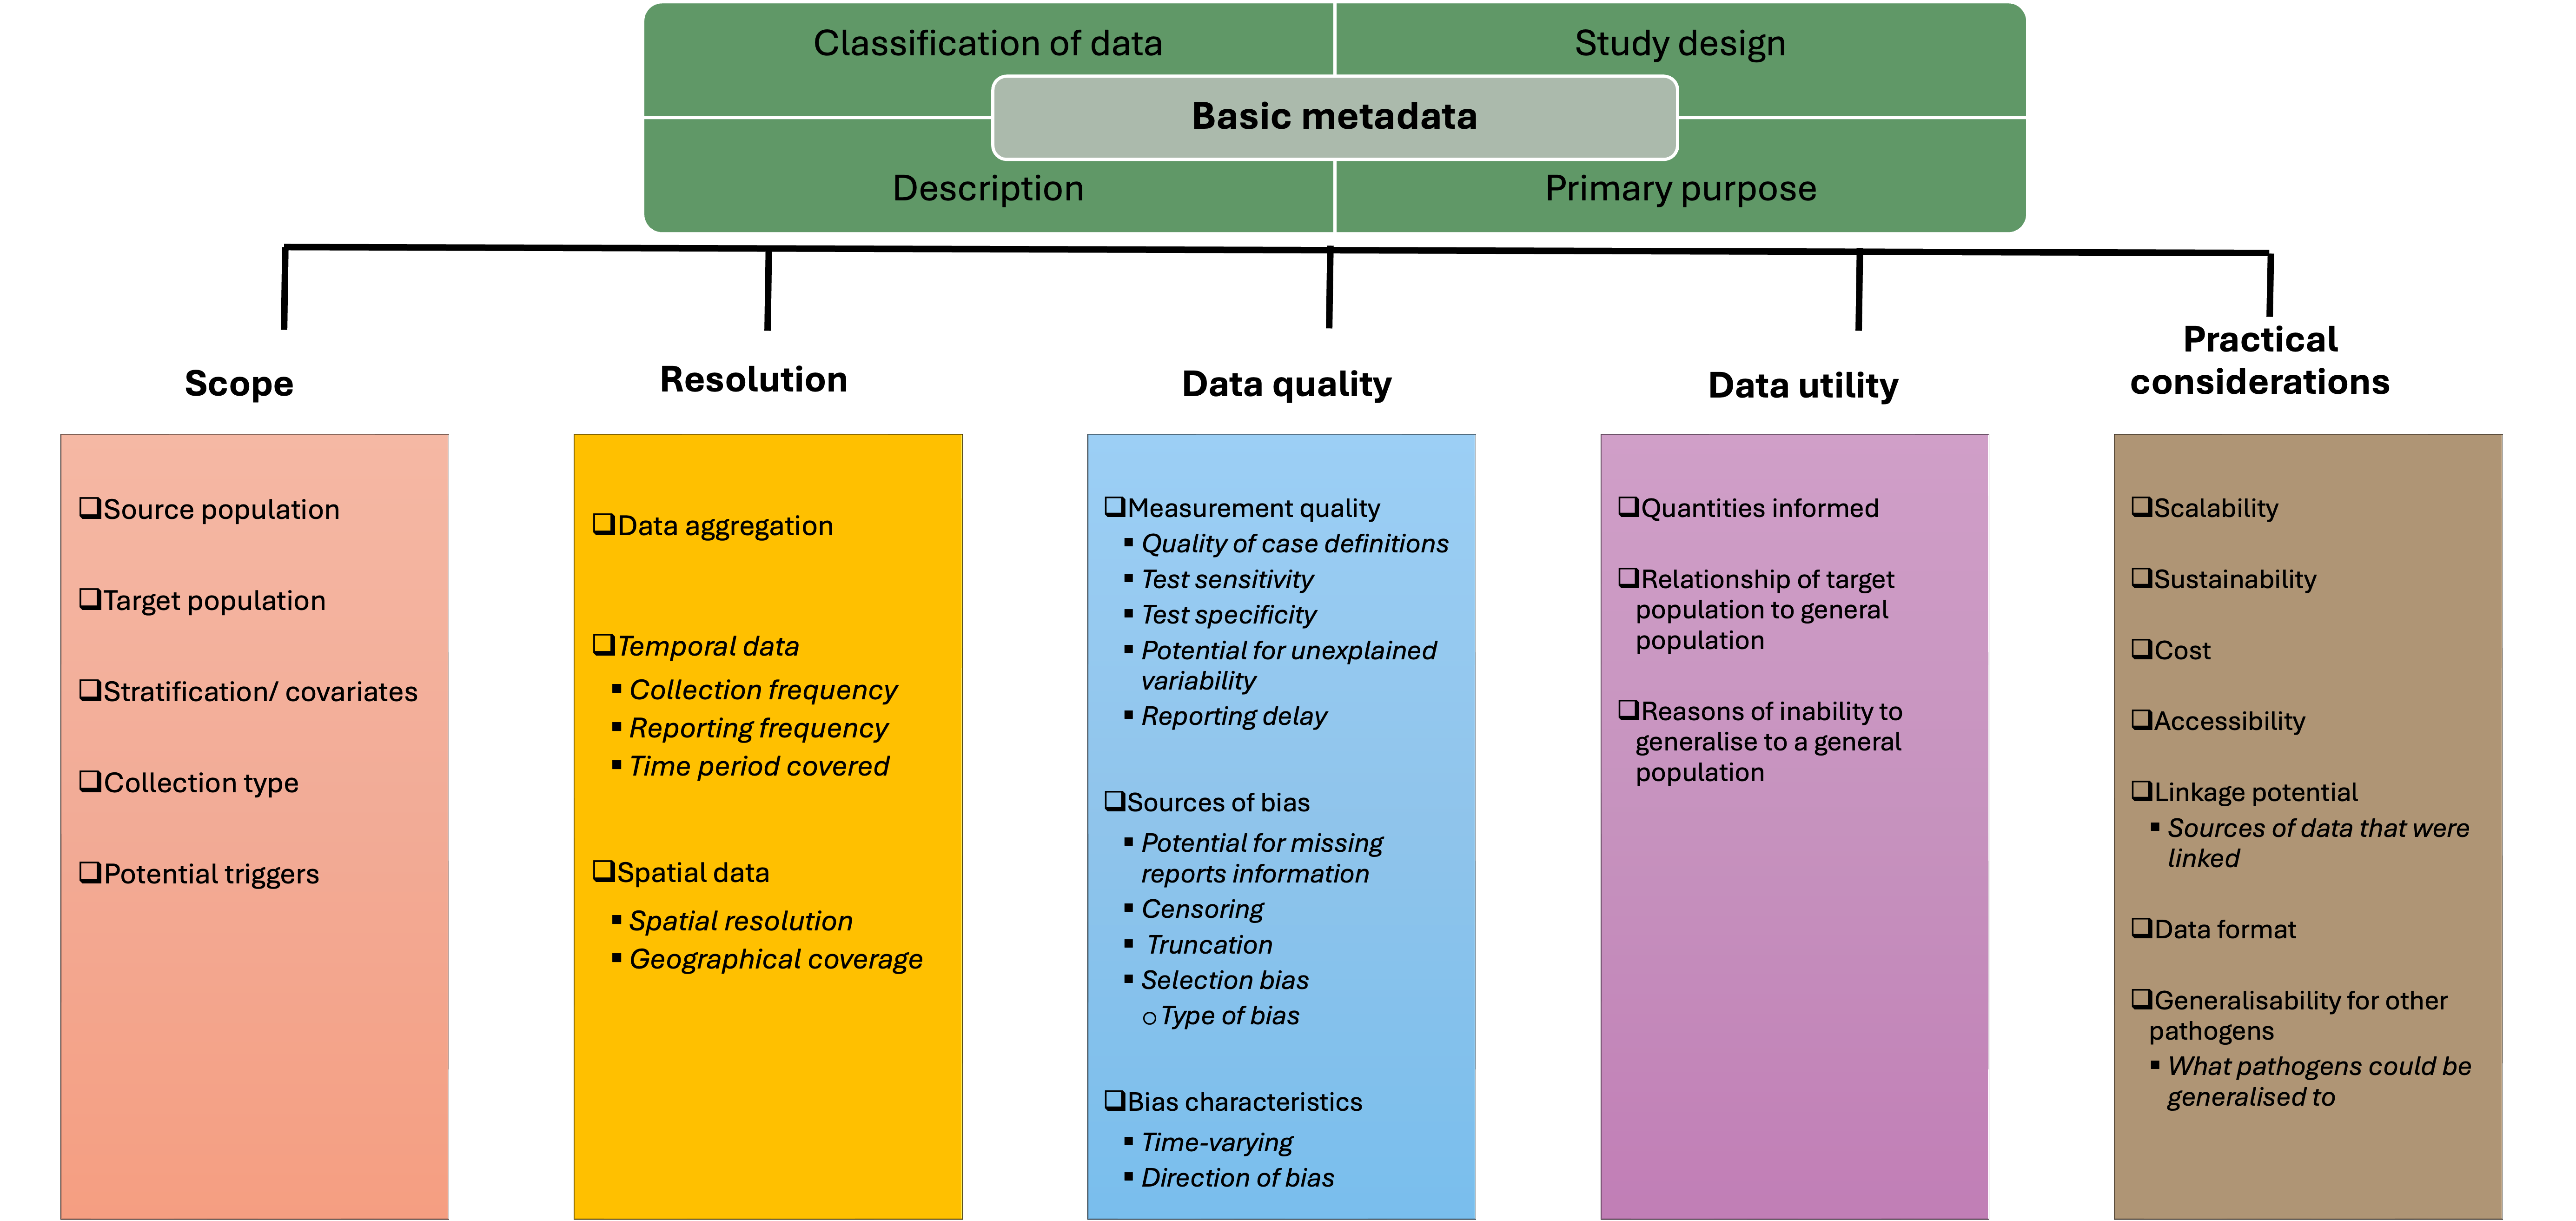
\includegraphics[width=1\linewidth]{figures/data_characteristics_2.png}
\centering
\caption{The proposed checklist for characterising a data stream used in infectious disease surveillance and modelling. The six core characteristics---metadata, scope, resolution, data quality, data utility and practical considerations---are illustrated alongside representative attributes that can be used to assess the strengths and limitations of each data source. }
\label{data_characteristics}
\end{figure}


\section{Workflow}
% Lead: Sam Abbott

\subsection{Overview}



\begin{figure}[htbp]
    \centering
    \includegraphics[width=\textwidth]{figures/core steps with more details.drawio.pdf}
    \caption{\textbf{Recommended workflow for integrating multiple data sources in infectious disease modelling.} Begin by defining research questions and target estimands, proceed through iterative development of process and observation DAGs, and follow critical decisions about data integration and inference methods. Key feedback loops from downstream parts of the workflow that impact earlier choices are represented with dashed arrows and boxes.}
    \label{fig:workflow}
\end{figure}

We recommend following a structured, iterative workflow for multi-data source modelling (Figure~\ref{fig:workflow}). Our suggested workflow extends established Bayesian workflow principles \citep{gelman2020bayesian} for  the specific challenges of multi-source infectious disease modelling.
We advocate this approach because it makes modelling choices transparent, assumptions explicit, and provides principled tools for assessing model adequacy regardless of whether final inference is Bayesian or frequentist.
The workflow should be implemented through multiple iterations, starting with high-level considerations and becoming more detailed with each pass, as some steps require later workflow components (e.g., posterior prediction requires inference and computation choices).

Begin with \textbf{decision making}: clearly define your research question and target estimands (e.g., time-varying reproduction number, overdispersion parameters).
Next, we suggest using \textbf{directed acyclic graphs (DAG)}  to define your models. However, we depart from standard approaches in that we suggest decoupling the definition of the \textbf{process} and \textbf{observation} models.
Here the \textbf{process model DAG} represents the underlying epidemiological process, i.e. the transmission and related processes.
A key part of this workflow is iterating on this representation as understanding develops i.e. during an outbreak.
The next step is to make use of the data source characterisation from the last section to \textbf{map available \textbf{data sources} }to your process model, such as incidence time series, genomic data, contact tracing, viral load measurements, and serological surveys based on those identified in the previous section.
Data sources should be selected based on their expected contributions to the research question.
For each data source, develop an \textbf{observation DAG} linking the underlying process to observed data through measurement models and reporting mechanisms.
Different data sources may also impact your \textbf{process DAG} assumptions, such as whether you can collapse your representation of the process from individual-level to population-level.

Once you have developed your \textbf{process} and \textbf{observation DAGs}, proceed to \textbf{model specification and validation}, including prior specification, parameter identifiability assessment, and prior predictive checks.
You then face key decisions on \textbf{data integration choices}: \textbf{``What to combine?''} and \textbf{``How to combine?''}.

If combining multiple sources is not beneficial or feasible, you can proceed to single-source modelling and potentially the combination of estimates, e.g. where multiple models estimate the effective reproduction number from different data sources, and so these estimates can be ensembled.
If integration is warranted, select among \textbf{data integration} methods. 
Once your data sources have been integrated, it is time to make \textbf{inference and computation choices}, i.e. selecting an inference method based on the model structure, integration approach, and theoretical and practical considerations. 
Finally, \textbf{fit your model} and evaluate its performance through posterior predictive validation and sensitivity analysis.

Throughout this workflow, there is the potential for feedback loops between steps so that model development is rarely a single forward pass (see Figure~\ref{fig:workflow}). 
Data characteristics can alter process DAG structure: individual-level data requires different representations than population-level data. 
Identifiability issues discovered during model specification may require simplifying either the process model or observation models. 
Practical constraints shape integration choices in multiple ways. Teams using incompatible programming languages may necessitate modular rather than joint approaches. 
Integration complexity itself may require simplifying observation models to maintain computational feasibility. Conflicts between data sources during integration often reveal model misspecification, requiring revision of earlier assumptions. 
Computational constraints during fitting may require approximating or restructuring the process DAG. Limited computational resources or available expertise may favour modular over joint integration approaches despite the theoretical advantages of joint modelling. 
For example, suppose you initially design a joint model but find it computationally intractable with available methods. In that case, you might iterate back to choose a modular integration approach, which in turn might influence how you structure your observation DAGs.

Practitioners should expect to repeat this workflow as outbreaks evolve.
Understanding of pathogen characteristics improves over time, research questions shift from immediate response to longer-term planning, and decision-making timescales change from days to months.
New data sources emerge whilst surveillance systems adapt to changing circumstances.
This evolution favours modular approaches that enable component reuse rather than bespoke models requiring complete redevelopment when applications change.
Critical to this workflow is transparent reporting of all decisions and validation procedures, including documentation of iterative workflow passes and decision rationales, enabling both reproduction and adaptation of models for future applications.

In the following sections, we will discuss each of these steps in more detail and provide resources for further learning. We will also demonstrate this workflow in our case studies.

\subsection{Research Question and Target Estimands}

Determining the research question shapes the entire modelling workflow, from data source selection through integration choices to validation strategies.
Start by engaging with policymakers and/or stakeholders to understand which epidemiological parameters matter for their decisions: some need simple short-term case forecasts for hospital planning, others require transmission dynamics understanding for intervention design \citep{marshall2024when}.
Often, multiple outcomes are desired that require balancing trade-offs: short-term forecasts for operational planning alongside $R_t$ estimates for public communication and interpretability.
The aim is to translate policy needs into specific target estimands by trying to understand how parameters inform decisions \citep{nicholson2022interoperability}.
For example, policymakers might need to know if transmission is increasing rather than precise values, or whether superspreading drives transmission, to choose between population-wide versus targeted interventions.
Try to define scope explicitly, including what the analysis cannot address: a national $R_t$ estimate cannot easily reveal local outbreak dynamics, aggregate case data might not be able to identify transmission chains, and surveillance might not be able to detect mild infections.
These limitations shape stakeholder expectations and prevent misuse of results.
Research questions evolve throughout outbreaks as understanding improves and policy needs shift.
Early outbreak questions often focus on growth rates and severity using limited case data.
As surveillance expands, questions might shift, for example, to variant dynamics requiring genomic integration, then to population immunity needing serological data.

\subsection{Process DAG Development} \label{sec:process}

Process DAG development translates research questions into formal causal structures that evolve throughout an outbreak.
A directed acyclic graph (DAG) represents causal relationships between variables through nodes (variables) and directed edges (causal influences), making assumptions explicit and testable \citep{digitale2022tutorial}.
This formalism helps identify confounders, mediators, and colliders that affect parameter estimation from observational data.
For infectious disease modelling, we recommend constructing DAGs that capture biological mechanisms: susceptible populations, transmission events, infection progression, recovery or death, and intervention effects \citep{deangelis2018analysing}.
Rather than starting from scratch, adapt established epidemiological models for similar pathogens or transmission routes, modifying components as outbreak-specific data emerges \citep{gelman2020bayesian}.
Begin with simple representations of core transmission dynamics, then iteratively refine as understanding improves during an outbreak.
Early outbreak DAGs might represent homogeneous mixing, while later versions incorporate age structure, spatial heterogeneity, or variant dynamics as data reveals their importance.
Key biological mechanisms drive DAG structure: incubation periods create delays between infection and infectiousness, viral load dynamics affect transmission probability, and immune waning influences reinfection risk.
We suggest separating process DAGs from observation DAGs to distinguish true epidemiological processes from how we measure them.
This separation enables modular model development where process components can be reused across different surveillance contexts \citep{nicholson2022interoperability}.

\subsection{Data Source Mapping}

Data source mapping connects available surveillance streams to epidemiological processes using the characteristics framework from Section~\ref{sec:datareview}.
After this systematic cataloguing of the available data,  it is then important to relate the strengths and weaknesses of each available data source to the target estimands.
Link data sources to process components by identifying what epidemiological quantities each stream measures. 
For example, cases reflect infection incidence with reporting delays and ascertainment bias, hospitalisations capture severe outcomes with admission thresholds, and wastewater indicates population-level viral circulation independent of healthcare-seeking.
Evaluate complementarity by examining whether sources provide independent signals or reinforce the same information.
For example, wastewater can potentially provide early warning of outbreaks, while clinical surveillance provides individual-level severity data.
Identify redundancy where multiple sources inform the same parameter, which might improve precision at the cost of model complexity.
Start with minimum data requirements for target estimands, then expand systematically.
Each additional source increases complexity and development time, so prioritise based on expected information gain relative to implementation cost \citep{jackson2019value,heath2024value}.
Document these mapping decisions explicitly as they shape all downstream workflow choices from observation DAG construction through integration methods.

\subsection{Observation DAG Construction} \label{sec:observation}

Observation DAGs map how latent epidemiological processes generate observed data, with complexity shaped by target estimands and available data sources \citep{deangelis2018analysing}.
Build these DAGs by working backwards from measured values through all intermediate steps: symptom onset, healthcare seeking, testing, laboratory processing, and reporting for clinical surveillance; viral shedding, sewage networks, and quantification for wastewater.
Each step introduces delays, biases, or missing data mechanisms that affect inference.
Treat observation components as modular and replaceable: initial Poisson noise models can become negative binomial, simple delays can incorporate weekly patterns \citep{gelman2020bayesian}.
This flexibility reduces initial specification burden whilst enabling systematic refinement.
The level of detail depends on research questions and later workflow choices.
Estimating population-level transmission requires simpler observation models than understanding variant-specific dynamics or age-stratified patterns.
Individual-level data enables different observation models compared to aggregated reports.
Model reporting and other delays explicitly as they create temporal misalignment between transmission events, disease sequelae and observations \citep{seaman2022nowcasting}.
Distinguish between missing data mechanisms since random missingness and systematic under-ascertainment require different handling \citep{sherratt2021exploring}.
Account for time-varying observation probabilities from testing capacity, healthcare seeking or surveillance intensity changes.
Account for hierarchical structure and population heterogeneity when multiple data sources capture different demographic subgroups.
Multiple observation DAGs for the same underlying process enable validation by checking whether different data streams imply consistent transmission dynamics when properly aligned.

\subsection{Iterate on the model DAGs}

After mapping data sources and constructing your observations DAGs, revisit your process and observations DAGs to ensure alignment between what you want to model and what your data can support.
Model development can begin simple and add complexity, or start comprehensive and simplify to essential components \citep{gelman2020bayesian}.
This step of the workflow aims to create a single joint DAG composed of your process and observations DAGs.
Data availability can drive both increases and decreases in model complexity.
Contact tracing data with identified transmission pairs enables shifting from population-level compartmental models to individual-based representations that capture heterogeneous mixing patterns.
Conversely, discovering that surveillance only provides aggregate counts may require collapsing a planned age-structured model into simpler compartments.
Strong prior information can sometimes compensate for data limitations, functioning almost like an additional data source.
For example, well-informed priors about transmission parameters from previous outbreaks might support maintaining a complex transmission model even when current data is limited and detailed knowledge about age-specific contact patterns from prior studies could support maintaining age structure, even with only total case counts.
Note that assuming fixed parameter values, common in mechanistic modelling literature, is effectively placing infinitely strong priors and should be avoided where possible in favour of appropriately uncertain prior distributions.
Temporal resolution affects what variation can be identified rather than what can be modelled: you can always build a daily-scale model, but weekly surveillance data will usually inform weekly or longer-term patterns, not daily fluctuations.
Additional DAG iteration typically occurs at key workflow stages, such as during model specification when identifiability issues emerge, during validation when misalignment between model structure and data patterns is exposed, during data integration, or due to practical or theoretical considerations related to model fitting (Figure~\ref{fig:workflow}) \citep{corbella2022inferring}.
Each iteration should address specific problems rather than making arbitrary changes.
Document why changes were made, preserving the rationale for future model extensions when better data or   more domain knowledge becomes available, or when computational methods improve.

\subsection{Model Specification and Validation}\label{sec:spec-validate}

Follow the systematic Bayesian workflow for model validation \citep{gelman2020bayesian}, working through structured phases that provide clear decision points and feedback loops.
Start by validating models in small subcomponents first, then explore combinations to identify integration challenges early.

\subsubsection{Prior Specification and Prior Predictive Checks}

Specify priors using domain knowledge where available through informative priors; otherwise, use weakly informative priors that regularise without dominating the likelihood.
Prior predictive checks simulate data from the prior to ensure model behaviour aligns with epidemiological plausibility before seeing data.
These checks can reveal several issues requiring model modification: unrealistic parameter ranges may indicate need for different priors or model constraints; implausible epidemic dynamics may suggest DAG structural changes; computational issues during simulation may indicate need for model approximations or reparameterisation.
When prior predictive checks reveal problems, return to DAG development (Sections \ref{sec:process} and \ref{sec:observation}) to simplify models, add model components, increase complexity through hierarchical structure, or implement approximations for computational tractability.
Prior specification problems may also indicate need for additional data sources or expert consultation to inform appropriate prior distributions.

\subsubsection{Model Fitting and Computational Validation}

After resolving prior predictive issues, fit the model using methods from Section \ref{sec:fitting}.
Validate computational aspects through diagnostic checks, fake data simulation, and simulation-based calibration where feasible.
Using simulated scenarios to validate parameter recovery provides valuable insights into model performance \citep{bouman2024bayesian}, whilst simulation-based calibration for each submodel provides stronger validation by verifying that inference algorithms can recover true parameters from simulated data \citep{talts2018validating}.
Address computational issues systematically: simplify model structure or increase prior informativeness if convergence fails; examine submodels in detail if joint fitting proves intractable; reparameterise models if mixing is poor; plot intermediate quantities like effective reproduction numbers to identify problematic components; run on data subsets or reduce iterations to speed up iteration; check for multimodality using multiple chains or parallel tempering.
Remember that the goal is to make predictions or learn about epidemiological processes, not merely achieve convergence of an arbitrary model \citep{gelman2020bayesian}.
If computational validation succeeds, provisionally accept the model for posterior validation.
Persistent computational issues require returning to model specification or considering alternative integration approaches (Section \ref{sec:integration}).

\subsubsection{Evaluate and Use Model}

Begin with posterior predictive checks to assess whether fitted models reproduce key features across all integrated sources.
These checks form the foundation of model validation by comparing model-generated predictions against observed patterns.
Apply cross-validation strategies, particularly leave-one-out and time-aware validation, to assess predictive performance whilst respecting temporal data structure.
Examine influence of individual data points and prior specifications through sensitivity analysis.

Assess parameter identifiability by examining whether data sources provide sufficient information to uniquely estimate target parameters; joint modelling often resolves identifiability issues that plague pipeline approaches \citep{lison2024generative, russell2024combined}.
For some models, formal structural identifiability approaches may be used to indicate where additional data or prior information is needed.
Implement poststratification as needed to correct for population representativeness issues.

Detect conflict between data sources, where different streams imply incompatible parameter values under the current model.
When conflict arises, use prior sensitivity analysis to quantify how much priors must change to accommodate observed data, revealing potential model misspecification or data quality issues \citep{roos2015sensitivity,nott2021approximation,kallioinen2021detecting}.
This conflict analysis connects directly to value of information assessments that prioritise data collection efforts \citep{jackson2019value}.

If posterior validation reveals model inadequacies, return to DAG development to modify model structure, add complexity, or implement different approximations.

\subsubsection{Model Comparison}

When multiple plausible model specifications exist, use Leave-One-Out Cross-Validation (LOO-CV), Watanabe-Akaike Information Criterion (WAIC), Continuous Ranked Probability Score (CRPS), or other methods to compare predictive accuracy \citep{vehtari2017practical,yao2018using,gneiting2007strictly} combined with visual posterior predictive checks.
High Pareto-k values from LOO-CV identify influential observations requiring careful modelling.
For infectious disease models, consider scoring transformations such as the log when using CRPS \citep{bosse2023scoring}.
Maximise sharpness subject to calibration: models should produce statistically consistent predictions whilst minimising required uncertainty \citep{gneiting2007strictly}.
Model comparison serves as the final validation step, ensuring that chosen specifications provide optimal predictive performance whilst maintaining epidemiological interpretability.

This approach creates multiple feedback loops with earlier workflow stages: prior predictive issues modify DAGs and data integration choices; computational problems may require approximations or different integration methods; posterior validation failures necessitate structural model changes.
For comprehensive implementation guidance, see \citep{gelman2020bayesian}.

\subsection{Data Integration Choices}\label{sec:integration}
% Lead: Anne Presanis

\subsubsection{Decision Framework}

In principle, integrating multiple data sources should enhance the identifiability and precision of parameter estimates \citep{deangelis2018analysing, lison2024generative, russell2024combined, birrell2025real}. Even when data streams are redundant (informing the same quantity), their combination can improve precision, consistent with meta-analytic principles \citep{deangelis2018analysing,borenstein2021introduction}. 

In practice, however, data integration may pose challenges. These include inconsistencies due to unaccounted biases \citep{presanis2013conflict,knock2021key, Ward2024-sp, corbella2022inferring}; computational complexity \citep{corbella2022inferring}; and real-time pressures during an outbreak emergency \citep{mccaw2023role}.

Evaluating the strengths and limitations of different data sources, as described in Section \ref{sec:datareview}, can and should be done during inter-epidemic periods. This evaluation, alongside the workflow of specifying process and observation DAGs (Section \ref{sec:process} and \ref{sec:observation}, helps assess whether estimands of interest are identifiable from the available data. Value-of-information methods \citep{jackson2019value,heath2024value} can formally guide whether new or additional data would meaningfully improve precision. However, for complex models especially, identifiability may only become evident after fitting an initial version.

Decisions about data integration are inherently context-dependent, but can be guided by the decision tree in Figure \ref{fig:integration}. When combining independent model outputs from different groups, the choice of ensembling or meta-analytic approach should align with the research objective (e.g. estimation or prediction), influencing how estimates or predictions are weighted (e.g. by precision or prediction accuracy). In contrast, when integrating sub-models, the approach will depend on whether existing sub-models have already been fitted or if the models are being developed de novo.

\subsubsection{Integration Methods}

\paragraph{Full joint modelling}

Specifying a full joint model of multiple data sources and the underlying processes generating them offers a coherent framework for integrating such sources simultaneously, in the spirit of Bayesian hierarchical models \citep{gelman2020bayesian}. This approach is especially suited when there are complex dependencies between data sources \citep{corbella2022inferring}, perhaps conditional on the parameters of the underlying process model, such that identification of all parameters is compromised when some data are left out. However, joint models can be computationally intensive and challenging to fit, especially in high-dimensional or real-time settings. Care is needed to ensure complex dependencies are appropriately modelled and that observational biases, such as selection biases, are adequately accounted for in the model, to avoid conflict between data sources \citep{presanis2013conflict,corbella2022inferring}. 

\paragraph{Modular approaches and staged fitting}
A modular model building approach \citep{deangelis2018analysing,goudie2019joining,gelman2020bayesian,nicholson2022interoperability} is generally recommended, guided by the principle of parsimony (``Occam's razor''). 
Starting with simple sub-models makes it easier to diagnose issues such as poor fit, model misspecification or convergence issues. Complexity can then be added incrementally, only as far as needed. Sequentially combining sub-models also facilitates the detection of inconsistencies or conflicts between them \citep{presanis2013conflict,manderson2023combining}. Modular approaches also offer computational advantages over joint modelling. Techniques like Markov melding \citep{goudie2019joining} allow posterior samples from one sub-model to serve as a proposal distribution for the next, potentially in a sequential chain of models \citep{manderson2023combining}. Similar sequential strategies, using the posterior from one sub-model as the prior (rather than proposal) for another, have a long history \citep{west1997bayesian}, closely related to Sequential Monte Carlo algorithms \citep{doucet2001introduction} (see Section \ref{sec:fitting}).

While the theory and some applications of Markov melding are well-established \citep{goudie2019joining,nicholson2022interoperability,manderson2023combining}, practical implementation remains challenging. Limitations include the availability of user-friendly Bayesian software and methods for assessing sub-model compatibility (REF). As a result, approximate methods are often used. A common approach is the one used in standard meta-analysis \citep{borenstein2021introduction} to combine previous estimates using a normal approximation. A Stage 1 point estimate, $\hat{y}_1$, and its corresponding standard error or posterior standard deviation $\hat{\sigma}^2_1$, can be incorporated in a Stage 2 model as a likelihood term, on an appropriate scale:
$$
\hat{y}_1 \sim N(\theta, \hat{\sigma}^2_1)
$$ for some parameter $\theta$ in the Stage 2 model informed by the Stage 1 estimate. This approach has been shown to be an approximation to Markov melding with ``product of experts'' pooling \citep{goudie2019joining}.

Modular approaches also support selective trust in sub-models. ``Cutting'' feedback -- i.e. preventing less reliable sub-models from influencing more trusted ones while allowing the reverse -- enables nuanced evidence synthesis \citep{plummer2015cuts,carmona2022scalable,yu2023variational,liu2025general}.

\paragraph{Ensembling independent models:} When multiple models target the same estimand, ensemble methods such as Bayesian stacking \citep{yao2018using}, model averaging \citep{hoeting1999bayesian}, or meta-analytical pooling \citep{jackson2011multivariate} can be used to combine estimates.
These differ from approaches like Markov melding in that they combine independent model outputs rather than partitioning a joint model into connected sub-models.
The choice of ensemble strategy should reflect the research objective.
For prediction, weighting by out-of-sample accuracy may be appropriate; for estimation, weights might reflect precision or model credibility \citep{yao2018using}.
Ensemble methods offer practical advantages when joint modelling proves infeasible, enabling collaboration between research teams and potentially improving robustness over single models.
The European COVID-19 Forecast Hub demonstrated performance gains from simple median aggregation \citep{sherratt2021exploring}, whilst the UK's SPI-M consensus used random-effects meta-analysis to pool Rt estimates from multiple academic groups \citep{manley2024combining}.

However, important limitations constrain ensemble approaches for infectious disease modelling.
When models make different assumptions about latent quantities, apparent heterogeneity may reflect definitional differences rather than true uncertainty about the estimand \citep{brockhaus2023why}.
Temporal alignment becomes particularly problematic for latent targets where the underlying definition remains ambiguous, with models using different reference points, generation time distributions, or reporting delay assumptions \citep{brockhaus2023why}.
This can lead to estimates that are less timely and/or less precise, with lower utility for decision makers than the component models \citep{manley2024combining}.
Combining outputs at the prediction level discards information about data conflicts and model disagreements that would be preserved in joint modelling approaches.
Weighted ensemble methods often show limited improvement over simple aggregation in nowcasting applications \citep{sherratt2021exploring}, partly because the black-box nature of many models obscures why predictions differ.

We recommend joint modelling, perhaps implemented via Markov melding or its approximations and making use of cut distributions if needed, when computationally and practically feasible. This type of integration enables coherent uncertainty quantification and avoids the definitional ambiguities that affect output-level combinations \citep{manley2024combining, brockhaus2023why}.
Ensemble methods remain valuable when joint modelling proves impossible due to computational constraints, data access limitations, or institutional boundaries between research teams.
When employing ensembles, careful attention to ensuring all models target the same estimand, resolving temporal alignment, and documenting methodological assumptions becomes essential for meaningful combination.


\subsubsection{Conflict Detection and Resolution}
% Prior-data conflict
% Data-data conflict
% Model criticism in multi-source settings
% Sensitivity analysis approaches

Detecting and resolving conflicting evidence about underlying latent processes is essential to ensure coherent inference and robustly informed decisions \citep{presanis2013conflict,sherratt2021exploring}. Such conflicts may arise between prior assumptions and data (``prior-data conflict''), between different data sources, between different partitions of a joint model into submodels, or even within a data source but between different units of data \citep{presanis2013conflict,yang2025detecting}.

If data sources and/or prior information provide inconsistent evidence on a parameter, this conflict usually manifests either as a lack of identifiability, a symptom of which may be lack of convergence of an MCMC algorithm or equivalent; or as lack of fit to one or more data sources \citep{presanis2013conflict,deangelis2018analysing}. Resulting estimates may therefore be more uncertain than if each data source were modelled independently. Such conflicts are typically the result of model misspecification: some observational bias that has not been accounted for in the observation model (e.g. under-reporting or selection bias); or some approximation in the process model that fails to explain the variation in the data (e.g. a fixed under-reporting proportion); or an unrealistic prior specification (e.g. an infection-fatality risk based on a previous pathogen which is not that similar to a newly emerging one).  

Diagnostic tools to detect conflicts in evidence synthesis models include prior-, mixed- and posterior-predictive checks, the latter often in a cross-validatory setting to avoid conservatism due to double use of the data \citep[][and references therein]{presanis2013conflict,yang2025detecting}; and extensions of these to latent levels of a hierarchical model \citep{yang2025detecting}. Once conflicts have been identified, they need to be resolved, through careful consideration of unaccounted biases or overly restrictive model assumptions (e.g. equi-dispersion) that may underlie the conflicts. Adjustments to the model structure may be needed, starting another cycle of the model development and criticism process. These adjustments might include loosening prior assumptions, weighting approaches to account for selection biases, and other bias modelling approaches \citep{deangelis2018analysing}.


% Copilot suggestion to flesh out the above in case useful:
%In multi-source modelling, detecting and resolving conflicts is essential to ensure coherent inference and robust decision-making. Conflicts can arise at various levels:
%Prior–Data Conflict: When prior beliefs are strongly contradicted by observed data, it may indicate misspecification or overly informative priors. Diagnostic tools such as prior predictive checks and posterior–prior overlap metrics can help identify such conflicts early in the modelling process.
%Data–Data Conflict: Different data sources may provide inconsistent evidence about the same underlying process, due to biases, measurement error, or contextual differences. Identifying these conflicts requires careful comparison of marginal likelihoods, posterior distributions, and model fit across data streams.
%Model Criticism in Multi-Source Settings: Traditional model criticism techniques—such as posterior predictive checks, residual analysis, and information criteria—must be adapted to account for the complexity introduced by multiple data sources. Modular approaches can help isolate problematic components, while joint models may require more sophisticated diagnostics.
%Sensitivity Analysis: Sensitivity analysis plays a key role in conflict resolution. Varying priors, data inclusion, or model structure can reveal the robustness of conclusions and help identify influential assumptions. In modular settings, sensitivity analysis can be performed component-wise, while in joint models, global sensitivity approaches may be more appropriate.
%Ultimately, conflict detection should be an iterative process, integrated into model development and refinement. Transparent reporting of conflicts and their resolution enhances the credibility and interpretability of modelling outputs, particularly in high-stakes settings such as outbreak response.


%\subsubsection{Practical Constraints}
% Different teams with different expertise/languages
% Software compatibility issues
% Computational resource limitations
% Time constraints in outbreak settings

% Copilot suggestion in case useful to flesh out the above:
% Despite the theoretical advantages of data integration and modular modelling, several practical constraints often limit their implementation in real-world settings:
%Diverse Teams and Disciplinary Silos: Collaborative modelling efforts frequently involve teams with varied disciplinary backgrounds, methodological preferences, and even programming languages. This diversity, while enriching, can complicate communication, model interoperability, and consensus on modelling frameworks.
%Software Compatibility: Differences in software ecosystems—such as R, Python, Stan, or proprietary tools—can hinder seamless integration of sub-models or data pipelines. Even when using the same language, variations in package versions or coding conventions can introduce friction.
%Computational Resources: High-dimensional models or those requiring extensive simulation (e.g., via MCMC) can be computationally demanding. Limited access to high-performance computing infrastructure may constrain the complexity or scale of models that can be feasibly implemented, particularly in low-resource settings.
%Time Constraints in Outbreak Settings: During public health emergencies, the need for rapid decision-making often precludes the development of fully integrated or optimised models. In such contexts, simpler or pre-existing models may be prioritised over more comprehensive but time-intensive approaches.
%These constraints highlight the importance of planning and infrastructure development during inter-epidemic periods, including the creation of interoperable modelling frameworks, shared codebases, and cross-disciplinary training.


\begin{figure}[htbp]
    \centering
    \includegraphics[width=\textwidth]{figures/integration choices decision tree.drawio.pdf}
    \caption{\textbf{Decision tree for integration choices when integrating multiple data sources in infectious disease model inference.} The flowchart guides researchers through key decision points to select appropriate integration strategies.}
    \label{fig:integration}
\end{figure}

\subsection{Inference and Computation Choices}\label{sec:fitting}
% Lead: Xiahui and Dhorasso with support from Anne Presanis

Inference for infectious disease models typically involves estimating a set of parameters $\theta$ from observed data $Y$, which may include case counts, hospitalisations, deaths, wastewater surveillance or other epidemiological measurements. These data are assumed to arise from a probabilistic model characterised by a likelihood function $p(Y | \theta)$ that links the parameters to the data through both an underlying transmission dynamics (represented by the process DAG (Section \ref{sec:process}) in our workflow) and a noisy observation mechanism (captured by the observation DAG (Section \ref{sec:observation})).  The choice of inferential approach depends on the tractability of the likelihood: 
whether $ p(Y | \theta)$ is analytically or numerically computable, intractable and requiring approximation, or entirely  unavailable (necessitating likelihood-free, simulation-based methods). 

A wide range of computational strategies exists for infectious disease model inference, with numerous methods and variants available for each broad class of approach.
We recommend structuring inference and computation decisions through four key considerations: assessing model complexity, selecting appropriate inference methods, implementing the chosen approach, and evaluating diagnostics (Figure \ref{fig:fitting}).
In addition, inference and computation choices involve critical feedback loops within the broader workflow: computational constraints may require approximating or restructuring the process and observation DAGs developed in earlier stages, whilst computational limitations or available expertise may favour modular rather than joint integration approaches, necessitating a return to data integration decisions.
Inference diagnostics may also reveal model specification issues necessitating a return to model specification and validation (Section \ref{sec:spec-validate}).
This section provides an overview of these considerations with detailed technical discussion and practical guidance for navigating the many available options.

\begin{figure}[htbp]
    \centering
    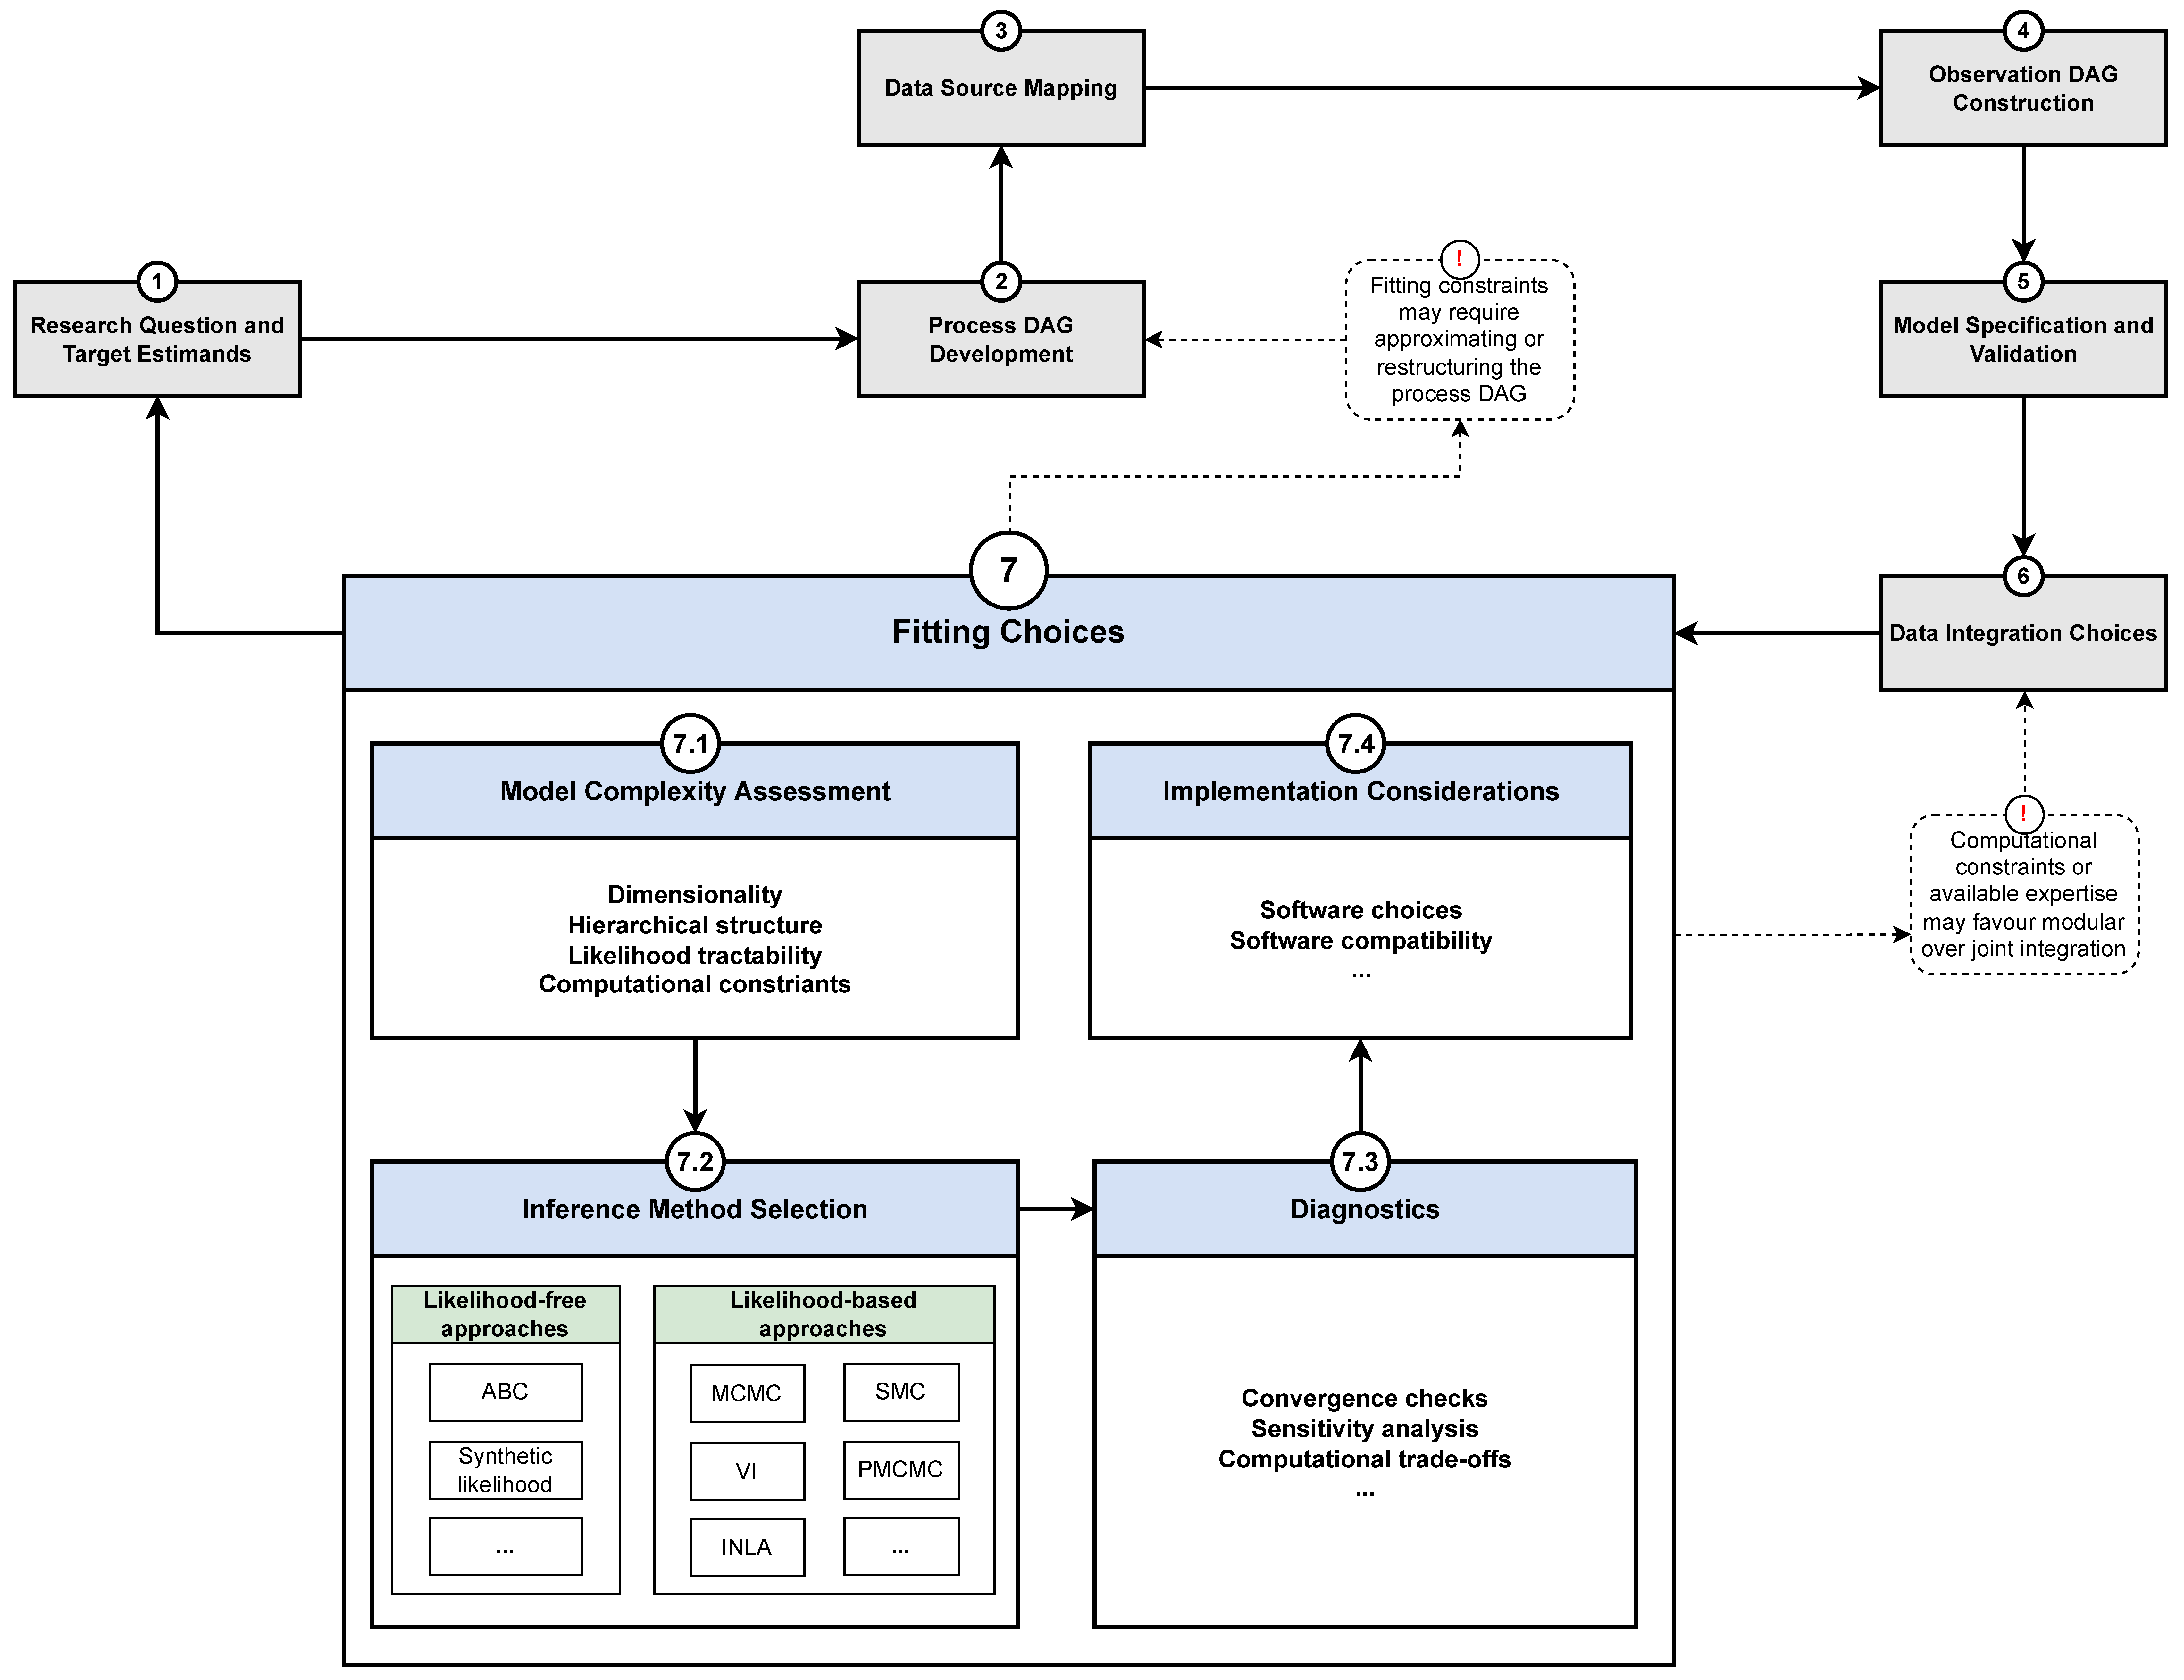
\includegraphics[width=\textwidth]{figures/subpanel_fitting choices.drawio.pdf}
    \caption{\textbf{Inference and computation choices workflow for integrating multiple data sources in infectious disease modelling.} The workflow contains four interconnected components: Model Complexity Assessment (7.1) evaluates dimensionality, hierarchical structure, likelihood tractability, and computational constraints; Inference Method Selection (7.2) chooses between likelihood-free approaches and likelihood-based methods; Diagnostics (7.3) involve convergence checks, sensitivity analysis, and computational trade-offs; and Implementation Considerations (7.4) address software choices and compatibility requirements. The interconnected arrows indicate that these components inform each other iteratively, allowing researchers to optimize the balance between model complexity, computational feasibility, and inferential accuracy when integrating multiple data sources. The workflow includes key feedback mechanisms: inference and computation constraints may require approximating or restructuring the process DAG, leading back to stage 2 Process DAG Development; computational constraints or available expertise may favour modular over joint integration approaches, requiring a return to stage 6 Data Integration Choices; diagnostic failures may indicate model specification issues requiring return to stage 5 Model Specification and Validation. }
    \label{fig:fitting}
\end{figure}


% \subsubsection{Likelihood-based methods}
% Likelihood-based inference encompasses frequentist and Bayesian approaches. Classical frequentist methods such as maximum likelihood estimation (MLE)\citep{myung2003tutorial, baltazar2024maximum} and profile likelihood \citep{tonsing2018profile, plank2024structured} provide well-established tools for parameter estimation. However, here we focus mainly on Bayesian methods due to their flexibility in handling uncertainty and incorporating various sources of information.

% Bayesian inference updates prior beliefs $ p(\theta)$ in light of observed data to obtain a posterior distribution $p(\theta | Y) \propto p(Y|\theta) \,p(\theta)$. For simple models with exponential family likelihoods, conjugate priors allow closed-form posterior solutions \citep{gelman1995bayesian,  cori2013new}. However, many infectious disease models involve complexities that preclude exact inference.

% When the likelihood can be evaluated (up to a constant) but closed-form posteriors are unavailable, sampling-based methods, especially Markov Chain Monte Carlo (MCMC) remain the gold standard \citep{gilks1995markov, lekone2006statistical}. Common algorithms include Metropolis–Hastings \citep{hastings1970monte} and Gibbs sampling \citep{geman1984stochastic}. For latent variable models, data-augmented MCMC introduces auxiliary states to jointly infer parameters and hidden variables \citep{o1999bayesian}. More efficient techniques, such as Hamiltonian Monte Carlo (HMC) for differentiable likelihoods \citep{duane1987hybrid} and its adaptive variant No-U-Turn Sampler (NUTS) \citep{hoffman2014no, andrade2020evaluation}, leverage gradient information for faster convergence and automatic tuning. 

% Alternatives to MCMC include Variational Inference (VI), which approximates the posterior by optimizing a tractable surrogate distribution, offering scalability at the cost of some bias \citep{blei2017variational, chatzilena2019contemporary}. Similarly, the Integrated Nested Laplace Approximation (INLA) 
% offers a computationally efficient method for approximating posterior marginals in latent Gaussian models, without relying on sampling-based methods \citep{rue2017bayesian}.

% In state-space models with high-dimensional latent state structures, the likelihood maybe intractable due to the need to marginalise over latent states. Sequential Monte Carlo (SMC) methods, or particle filters, approximate the posterior using weighted particles and yield unbiased likelihood estimates \citep{doucet2001introduction}. These can be embedded within MCMC to form particle MCMC (PMCMC) \citep{andrieu2010particle, endo2019introduction} , enabling joint parameter and latent state inference. Sequential Monte Carlo Squared (SMC$^2$) \citep{chopin2013smc2} extends this to fully sequential Bayesian updating as new data are accumulated.

% \subsubsection{Likelihood-Free Methods}

% Likelihood-based methods are powerful for parameter inference but rely on evaluating the likelihood function, which is sometimes infeasible for complex infectious disease models. Likelihood-free methods circumvent this by simulating from the model instead.

% Approximate Bayesian Computation is a popular likelihood-free method that approximates the posterior distribution by accepting parameter values that generate simulated data close to the observed data under a predefined distance metric \citep{rubin1984bayesianly, tavare1997inferring, beaumont2002approximate}. While conceptually simple, the classical ABC rejection sampling is inefficient in high-dimensional settings, prompting the development of more advanced variants. 

% ABC-MCMC combines ABC with MCMC to improve sampling efficiency, especially for peaked or correlated posteriors \citep{marjoram2003markov, wegmann2009efficient, kypraios2017tutorial}. However, its performance is sensitive to the choice of tolerance thresholds and proposal distributions.

% ABC-SMC further enhances efficiency by iteratively refining  tolerances and proposal distributions, adaptively focusing computational effort on high-probability regions and handling multi-modal posteriors more effectively \citep{sisson2007sequential, toni2009approximate, beaumont2009adaptive, drovandi2011likelihood}. 

% When exact likelihoods are unavailable but the model can be simulated repeatedly, synthetic likelihood methods provide an alternative by approximating the likelihood via assuming Gaussian distributions for summary statistics \citep{wood2010statistical, price2018bayesian}. 

% \subsubsection{Selecting the Right Tool}

% Selecting an appropriate inference method involves balancing trade-offs between computational efficiency, statistical rigor, data availability, interpretability, and model complexity \citep{funk2020choices}. Rather than adopting a universal approach, the choice should be tailored to the specific modelling context and inferential goals. 

% For evolving epidemics, a key consideration is the dynamic nature of epidemic processes and data streams. As transmission rates and intervention effects change over time, and new data arrive continuously, methods that support sequential data updates, such as SMC, are generally preferred for real-time epidemic tracking \citep{birrell2020efficient, storvik2023sequential}. In contrast, MCMC-based methods, while statistically robust, are typically better suited for retrospective analyses, due to their reliance on complete datasets, high computational demands for reanalysis, and computational intensity in high-dimensional parameter spaces. 

% When computational resources are constrained, for example during real-time outbreak monitoring or when analyzing large datasets, approximate methods like VI or ABC-SMC might offer scalable alternatives \citep{chatzilena2019contemporary, engebretsen2023real}. VI is highly scalable and typically much faster than MCMC, although it trades accuracy for speed and may not always be suitable where posterior uncertainty is important. Likelihood-free methods, while offering flexibility for complex models, tend to be computationally expensive because of repeated model simulation.

% Beyond computational efficiency, statistical accuracy is influenced by algorithmic choices including priors distributions, tuning parameters, tolerance thresholds, and the number of particles or iterations. Full-likelihoods methods typically yield better estimator performance, subject to likelihood tractability and proper specification, whereas likelihood-free approaches often prioritise flexibility and scalability over precision \cite{alahmadi2020comparison}. 

% Interpretability and ease of implementation also play a role. Certain methods integrate smoothly with probabilistic programming environments, while others may require further tuning and computational expertise. Ultimately, method selection should follow a systematic decision process that considers modeling goals, urgency or latency constraints, system complexity, and available computational resources. 

% Regardless of the approach chosen, model checking, sensitivity analysis, and validation are essential to ensure that inferences are not only statistically valid but also scientifically meaningful and actionable.

% NOTE: The following content on generative model validation should be relocated to model validation section:
% - Content about using fully generative PPLs for simulation-based calibration
% - Discussion of sampling from models without separate generators
% [TO BE MOVED: "Using a fully generative probabilistic programming language like Turing.jl or NumPyro makes model validation such as simulation-based calibration easier, as one can easily sample from the model without writing separate model generators required when using other approaches."]

\subsubsection{Model Complexity Assessment}

Inference for infectious disease models typically involves estimating a set of parameters $\theta$ from observed data $Y$, which may include case counts, hospitalisations, deaths, wastewater surveillance or other epidemiological measurements.
These data are assumed to arise from a probabilistic model characterised by a likelihood function $p(Y | \theta)$ that links the parameters to the data through both an underlying transmission dynamics (represented by the process DAG in our workflow) and a noisy observation mechanism (captured by the observation DAG).
Bayesian inference updates prior beliefs $p(\theta)$ in light of observed data to obtain a posterior distribution $p(\theta | Y) \propto p(Y|\theta) \,p(\theta)$, providing a principled framework for uncertainty quantification even when using non-Bayesian fitting methods.

Parameter dimensionality and structure represent key characteristics to assess.
Low-dimensional problems (fewer than 10 parameters) differ fundamentally from high-dimensional parameter spaces (hundreds or thousands of parameters), with method performance varying substantially across this dimension (see "Handles high-dim. params.?" in Table \ref{tab:methods_comparison}).
Parameter structure also matters: strongly correlated parameters, discrete parameter spaces, or mixed continuous-discrete problems each present distinct challenges.

Likelihood tractability determines which broad classes of methods are feasible.
Key questions include: Can the likelihood $p(Y | \theta)$ be written down analytically?
If not analytical, can it be evaluated numerically with reasonable computational cost?
Can the likelihood be differentiated with respect to parameters?
Many infectious disease models involve complexities such as stochastic differential equations or discrete event processes that affect tractability.

The presence and scale of latent states represents another structural consideration.
Models may include unobserved infection times, individual-level disease states, or spatially varying transmission rates.
The dimensionality of these latent structures relative to observed data affects computational feasibility.

Computational budget constraints frame practical considerations.
Real-time outbreak analysis demands different approaches than retrospective studies, with some methods supporting real-time inference whilst others require complete datasets (see "Capable of real-time inference?" in Table \ref{tab:methods_comparison}).
Available computational resources, from laptops to high-performance clusters, set practical limits.

\subsubsection{Inference Method Selection}

Numerous inference methods and algorithmic variants exist within each broad class of approach, each with distinct computational characteristics and practical trade-offs.
Selecting an appropriate method involves balancing considerations of computational efficiency, statistical rigour, data availability, interpretability, and model complexity.
Rather than adopting a universal approach, the choice should be tailored to the specific modelling context and inferential goals.
The following provides guidance for navigating these many options.

Gradient-based Markov Chain Monte Carlo (MCMC) approaches represent our preferred methods when applicable due to their combination of efficiency, reliability, and ease of use.
MCMC methods generate samples from the posterior distribution by constructing a Markov chain that converges to the target distribution, providing a flexible framework for Bayesian inference when analytical solutions are unavailable.
Hamiltonian Monte Carlo (HMC) leverages gradient information for efficient MCMC exploration of differentiable likelihoods, with its adaptive variant No-U-Turn Sampler (NUTS) representing our default recommendation for models with continuous parameters \citep{duane1987hybrid, hoffman2014no, andrade2020evaluation}.
These methods provide excellent diagnostics and automatic tuning, reducing the expertise barrier for reliable implementation.
When implementing gradient-based methods, automatic differentiation backend selection matters: forward-mode differentiation suits models with few parameters (typically fewer than 10), whilst reverse-mode differentiation scales better for high-dimensional parameter spaces.
Practitioners should test available autodiff options when possible, with systems like Turing.jl and PyMC providing backend flexibility.
When full uncertainty quantification is less critical, Variational Inference (VI) approximates the posterior by optimising tractable surrogate distributions, offering fast approximation with modern variants like Pathfinder \citep{blei2017variational, chatzilena2019contemporary}.

Sampling-based approaches become necessary when gradients are unavailable.
Standard Markov Chain Monte Carlo (MCMC) methods including Metropolis-Hastings and Gibbs sampling handle discrete or mixed parameter spaces \citep{hastings1970monte, geman1984stochastic, gilks1995markov}.
For discrete parameters, consider whether marginalisation is possible before resorting to sampling, as analytical integration can significantly improve efficiency and mixing.
Parallel tempering extends these methods to multimodal posteriors by running multiple chains at different temperatures, with modern implementations available in packages like Pigeons.jl \citep{surjanovic2023pigeons}.
These approaches require greater tuning than gradient-based methods and provide weaker diagnostics.

Sequential and particle methods suit dynamic models with high-dimensional latent states.
These approaches excel when models involve state-space formulations where latent states evolve over time and must be estimated alongside parameters.
Sequential Monte Carlo (SMC) methods, or particle filters, approximate the posterior using weighted particles and enable state estimation in high-dimensional spaces with strong real-time capabilities \citep{doucet2001introduction}, making them particularly valuable for real-time epidemic tracking where new data arrive continuously.
Particle MCMC (PMCMC) embeds SMC within MCMC to enable joint parameter-state inference \citep{andrieu2010particle, endo2019introduction}.
Important limitations include particle degeneracy (when few particles carry most weight), memory scaling challenges with long time series, and complex resampling tuning.
Table \ref{tab:methods_comparison} shows their moderate performance with high-dimensional parameters despite strength in latent state estimation.

Likelihood-free approaches serve as methods of last resort due to their computational demands and limited diagnostic capabilities.
These simulation-based methods bypass likelihood evaluation entirely, instead using model simulations to approximate the posterior distribution.
Approximate Bayesian Computation (ABC) approximates the posterior distribution by accepting parameter values that generate simulated data close to the observed data under a predefined distance metric, whilst synthetic likelihood methods approximate the likelihood by assuming Gaussian distributions for summary statistics \citep{beaumont2002approximate, wood2010statistical, price2018bayesian}.
Whilst these methods suffer from limited diagnostics and high computational cost, they provide essential flexibility for complex models where other approaches fail.

Approximate Bayesian methods provide efficient alternatives for specific model structures.
Integrated Nested Laplace Approximation (INLA) offers a computationally efficient method for approximating posterior marginals in latent Gaussian models, making it particularly effective for spatiotemporal disease models with spatial correlation structures \citep{rue2017bayesian}.
This method excels when models can be reformulated with latent Gaussian components but struggles with non-Gaussian latent structures.
Nested Laplace approximations can be integrated within other sampling schemes, allowing INLA to handle subcomponents of larger models efficiently.

Deterministic approaches focus on point estimation rather than uncertainty quantification.
Maximum Likelihood Estimation (MLE) provides point estimates for model parameters, particularly useful for simple models requiring only parameter estimates rather than full uncertainty quantification \citep{myung2003tutorial, baltazar2024maximum}.
Profile likelihood methods extend MLE by examining the likelihood surface for individual parameters whilst optimising over others, providing confidence intervals without full posterior sampling \citep{tonsing2018profile, plank2024structured}.
Whilst we do not generally recommend these approaches for primary analysis, they can prove useful for model validation, parameter initialisation, or exploring model behaviour when more complex methods encounter difficulties.

Our recommended approach follows a decision hierarchy:
First, attempt gradient-based MCMC (HMC/NUTS) for continuous parameter models with tractable, differentiable likelihoods.
When discrete parameters are present, use standard MCMC with parallel tempering for multimodal posteriors.
For state-space models with high-dimensional latent states, consider SMC/PMCMC despite their limitations.
When models have Gaussian latent field structure, INLA may outperform sampling methods.
Reserve likelihood-free methods for cases where likelihood evaluation proves impossible.

\begin{landscape}
\begin{table}[ht]
\renewcommand{\arraystretch}{1.2}
\centering
\caption{\textbf{Comparison of Likelihood-Based and Likelihood-Free Fitting Methods.} 
This table focuses on foundational algorithms. More recent methodological advancements that build upon these classical approaches are discussed in Section 4.9 of the main text. ``PPL'' stands for Probabilistic Programming Languages. For this review, PPL examples include Stan, PyMC, JAGS, NIMBLE, Turing. jl, etc.}
\label{tab:methods_comparison}
\small
\begin{tabular}{@{}p{3.2cm}p{1.5cm}p{1.5cm}p{1.5cm}p{1.5cm}p{1.5cm}p{1.5cm}p{1.5cm}p{1.5cm}@{}}
\toprule
\multirow{2}{*}{\textbf{Feature}} & \multicolumn{6}{c}{\textbf{Likelihood-Based}} & \multicolumn{2}{c}{\textbf{Likelihood-Free}} \\
\cmidrule(lr){2-7} \cmidrule(lr){8-9}
 & MLE & MCMC & PMCMC & SMC & INLA & VI & ABC & BSL \\
\midrule
\textbf{Theoretical Considerations} & & & & & & & & \\
\midrule
Requires likelihood? & Yes & Yes & Yes & Yes & Yes & Yes & No & No \\
Handles high-dim. params.? & Poor & Moderate & Moderate & Moderate & Good & Good & Moderate & Moderate \\
Convergence guarantees & Asymptotic & Asymptotic & Asymptotic & Asymptotic & Approx. & Approx. & Approx. & Approx. \\
Distributional flexibility & Low & High & High & High & Medium & Medium & High & Medium \\
Approximation error & Exact (asymp.) & Exact (asymp.) & Exact (asymp.) & Particle-based & Deterministic & Variational & Simulation & Simulation \\
\midrule
\textbf{Practical Considerations} & & & & & & & & \\
\midrule
Computational cost & Low & High & Very high & Med--High & Low & Low--Med & High & High \\
Scalability (big data) & Good & Poor & Poor & Moderate & Good & Good & Moderate & Moderate \\
Example software & PPL & PPL & POMP, NIMBLE & LibBi & R-INLA & PPL &abctools, EasyABC, ELFI & ELFI \\
Tuning required? & Minimal & Step size, priors & Complex & Resampling & Minimal & ELBO opt. & Sum. stats., distance, threshold & Sum. stats. \\
Capable of real-time inference? & Yes & No & No & Yes & Yes & Yes & No & No \\
Parallelization potential & 
High & 
Limited, chain-level, GPU possible but hard & 
Limited, particle-level, GPU possible for simple models & 
High, particle-level, GPU possible & 
Low, matrix operation hard to parallelise & 
Medium, gradient parallelisation; GPU possible & 
High, simulations parallelisable; GPU possible & 
Medium, GPU possible \\
Best use case & Simple models & General Bayesian inference & State-space models & Real-time inference & Latent Gaussian models & Fast approximation & Intractable likelihood & Intractable likelihood + summary stats \\
\bottomrule
\end{tabular}
\end{table}
\end{landscape}

Table \ref{tab:methods_comparison} provides detailed comparison across multiple criteria to support these decisions.

\paragraph{Hybrid and Nested Approaches}

Modern probabilistic programming languages enable sophisticated combinations of inference methods.
INLA approximations can be nested within NUTS, using efficient spatial approximations while sampling other parameters.
Languages like Turing.jl support mixed samplers, applying HMC to continuous parameters whilst using Gibbs for discrete components.
SMC methods can incorporate HMC kernels for parameter moves, leveraging particle filtering for states and gradient-based sampling for parameters.
These hybrid approaches capitalise on the strengths of multiple methods.

When complex methods fail to initialise properly within prior bounds, simpler methods can provide starting values for more sophisticated approaches.
Variational Inference often proves effective for initialisation due to its speed and robustness, whilst MLE can provide reasonable point estimates.
However, initialisation difficulties may indicate unrealistic prior specifications, suggesting model validation should be revisited before proceeding with complex inference.

\subsubsection{Implementation considerations}

A wide range of software tools is available to support the implementation of both likelihood-based and likelihood-free methods in infectious disease modeling (Table \ref{tab:methods_comparison} provides specific software examples for each method). Bayesian inference platforms such as Stan, JAGS and NIMBLE are widely used for likelihood-based approaches, offering flexibility in model specification and efficient MCMC algorithms \citep{carpenter2017stan,abril2023pymc}. For more complex or high-dimensional models, Python based PyMC and Julia-based Turing.jl provide probabilistic programming environments with good performance \citep{abril2023pymc,ge2018turing,fjelde2025turing}. For more scalable alternatives to MCMC, INLA is implemented in the R-INLA package \citep{martins2013bayesian} and is particularly efficient for latent Gaussian models, including spatiotemporal structures commonly used in disease mapping and surveillance. VI is also available in PyMC and Turing.jl. These implementations allow rapid inference for large datasets or real-time modelling applications.  Additionally, tools such as LibBi support SMC-based inference for state-space models and can scale to high-dimensional problems using GPU and parallel computing \citep{murray2015bayesian}. For likelihood-free methods, ABC is supported in packages like EasyABC, abc, abctools \citep{jabot2013easy,csillery2012abc,nunes2015abctools}.

The tuning burden varies substantially across inference methods, influencing both implementation time and reliability (see "Tuning required?" row in Table \ref{tab:methods_comparison}) \citep{funk2020choices}.
HMC and NUTS require minimal manual tuning due to automatic step size adaptation and mass matrix estimation, making them accessible to practitioners with limited MCMC experience.
Standard MCMC methods demand careful tuning of proposal distributions, step sizes, and mixing parameters, often requiring extensive pilot runs and convergence diagnostics.
Particle methods introduce additional complexity through particle count selection, resampling thresholds, and proposal kernel tuning.
ABC approaches require the most extensive tuning, involving summary statistic selection, distance metric choice, and tolerance threshold optimisation, often necessitating substantial methodological expertise.
INLA and VI require less runtime tuning but may need model reformulation to fit within their respective frameworks.

Parallelisation becomes essential for large-scale epidemiological studies, where high-performance computing resources are often required to handle complex models and extensive datasets.
MCMC methods (including HMC, NUTS, Metropolis-Hastings, and Gibbs sampling) face inherent parallelisation challenges due to their sequential chain structure, though multi-chain parallelisation provides the primary scaling mechanism and parallel tempering naturally exploits multi-core architectures through temperature-parallel chains \citep{surjanovic2023pigeons}; some implementations support within-chain parallelisation for specific operations (Stan and Turing.jl for gradient calculations, GPU acceleration for matrix operations), though memory access patterns and conditional branching make GPU implementations challenging.
VI scales exceptionally well through mini-batch parallelisation and routinely uses GPU acceleration for large datasets \citep{hoffman2013stochastic, bingham2019pyro}.
Sequential and particle methods excel at parallelisation through particle-level parallelism across CPU cores or GPU threads, with modern GPU architectures enabling thousands of particles to process simultaneously, though memory requirements scale with particle count \citep{henriksen2012parallel}.
Approximate methods show mixed potential: INLA has limited opportunities due to sequential matrix operations, though some implementations exploit parallel linear algebra libraries and nested approximations can parallelise across spatial or temporal components when model structure permits.
Likelihood-free methods provide excellent opportunities as ABC simulations parallelise trivially across CPU clusters and GPU architectures, though memory requirements can become substantial for large simulated datasets \citep{kulkarni2022hardware}, whilst synthetic likelihood approaches enable GPU acceleration for density estimation.
Deterministic approaches parallelise most effectively, with MLE highly parallelisable across data points on both multi-core CPUs and GPUs, and profile likelihood calculations naturally parallelising across parameter values.
When selecting methods for high-performance computing environments, practitioners should weigh these parallelisation capabilities (detailed in Table \ref{tab:methods_comparison}) against memory constraints, available hardware, and computational demands specific to their epidemiological applications.


\subsubsection{Diagnostics}

The quality and availability of diagnostic tools varies substantially across inference methods, representing a key factor in method selection.
Methods with better diagnostics are easier to use reliably, particularly for practitioners without extensive computational expertise.

HMC and NUTS provide the gold standard for diagnostic information.
Divergences indicate when the sampler fails to explore the posterior accurately, whilst the Bayesian Fraction of Missing Information (BFMI) diagnoses inefficient exploration of the typical set.
Traditional MCMC diagnostics including $\hat{R}$ and effective sample size (ESS) complement these HMC-specific metrics.
Energy plots and treedepth warnings provide additional insight into sampler performance.

Standard MCMC methods rely on traditional diagnostics including trace plots and $\hat{R}$ statistics.
Whilst useful, these provide less reliable indications of convergence than HMC diagnostics.
Visual inspection of trace plots remains important but can miss subtle convergence failures.

Parallel tempering adds temperature swap acceptance rates as key diagnostics.
Poor mixing between temperatures indicates inadequate exploration of multimodal posteriors.
Standard MCMC diagnostics apply to each temperature chain.

SMC and PMCMC methods use effective sample size of particles as the primary diagnostic.
Particle weight degeneracy indicates when resampling becomes necessary.
Sequential diagnostics track particle diversity over time, crucial for long time series.

Variational Inference provides limited diagnostic information through ELBO convergence monitoring.
However, ELBO convergence does not guarantee accurate posterior approximation.
Posterior predictive checks become essential for validation given limited intrinsic diagnostics.

ABC methods offer minimal diagnostic capabilities.
Acceptance rates and summary statistic distributions provide limited insight into approximation quality.
Heavy reliance on posterior predictive checks and external validation becomes necessary.

INLA provides model-specific diagnostic checks including residual analysis for latent Gaussian models.
Marginal likelihood approximations enable model comparison but do not diagnose convergence issues.

Diagnostic failures may indicate model specification issues requiring return to validation procedures (Section \ref{sec:spec-validate}).
For example, when using NUTS, divergent transitions suggest posterior geometry problems requiring structural model changes.

\subsection{Outbreak Evolution and Workflow Iteration}
% Lead Sam Abbott
Two types of changes during outbreaks require revisiting this workflow.
First, new information emerges about pathogen characteristics, surveillance capabilities, and population dynamics that may necessitate updating model assumptions and data integration choices \citep{mccaw2023role}.
Second, research questions evolve as outbreak priorities shift from initial detection and characterisation towards intervention evaluation and long-term planning.
When these changes occur, practitioners should iterate through the workflow, visiting their earlier decisions, rather than developing entirely new models.

Changes that warrant workflow iteration include: substantial new data sources becoming available (such as genomic surveillance or serological surveys); shifts in research questions that alter target estimands; and improved understanding of pathogen biology that changes process model assumptions \citep{knock2021key}.
The modular approach we advocate enables practitioners to update specific workflow components whilst preserving elements from previous iterations.
For example, observation models developed for case surveillance can often be reused when adding death reporting, whilst process models for transmission dynamics may require updating when new variants emerge.
This incremental approach reduces development time and maintains continuity across evolving outbreak contexts.

These steps are often carried out on an ad-hoc basis by teams during outbreaks but we think that a more formal approach that tracks decisions is likely to improve the quality of models produced and be ultimately less resource-intensive.
Establishing regular review points to assess whether workflow iteration is needed is likely to be beneficial with more regular reviews during acute outbreak phases.
Each iteration should document what has changed, why updates are necessary, and how new approaches build upon previous work.
Having this documentation supports both real-time decision-making and retrospective evaluation of analytical approaches.

\subsection{Workflow Reporting}
% Lead Sam Abbott
Complex multi-source models require clear documentation to enable evaluation and reproduction.
Without structured reporting, even well-designed workflows are difficult to assess or improve upon.

Visual schematics should communicate model architecture.
Process and observation DAGs should be reported separately, with integration methods explicitly diagrammed if multi-step methods are used.
For example, Ward et al.'s analysis of COVID-19 hospitalisation and fatality risk provides useful visual communication of model relationships but would benefit from process DAGs and code availability \citep{Ward2024-sp}.

Validation procedures should be documented comprehensively: prior and posterior predictive checks, conflict detection, and sensitivity analyses.
Abbott et al.'s COVID-19 Delta variant analysis demonstrates reporting with code, data and posterior predictions, though it lacks prior predictive checks and integration conflict discussion \citep{Abbott2021-delta}.
Readers cannot fully assess model performance without diagnostic outputs, as illustrated by recent preprints where validation procedures are unreported \citep{Fyles2024-qz}.

Code should be shared alongside results because it enables verification and accelerates progress.
For example, Abbott et al.'s prevalence estimation work has complete GitHub code, with clear links to model verification utilities, alongside the write-up \citep{Abbott2022-prevalence}.
Not sharing code, sharing it on request \citep{Ward2024-sp}, or only once a paper is in a peer-reviewed journal \citep{Fyles2024-qz} all create barriers to assess data integration workflows.

When data cannot be shared, synthetic data generation helps readers understand model behaviour.
For example, Mellor et al.'s norovirus nowcasting study provides training data with statistical noise added to preserve anonymity \citep{Mellor2025-noroviru}.
Progressive disclosure is preferable to indefinite withholding.
Even incomplete sharing - mathematical specifications, validation code, synthetic examples - supports scientific progress.

Throughout our workflow, we emphasise making decisions transparent at each stage.
These decisions should be reported alongside the results from the work, including rationales for data source selection, integration method choices, model structure assumptions, and validation procedures undertaken.
This reporting enables both evaluation of current work and informed adaptation for future applications.

Ideally, version control should be used for workflow development with the full git history available to demonstrate how models evolved during development.
Even more ideally, to gain trust, the full analysis should be public as much as possible at all stages \citep{Abbott2021-delta, Abbott2022-prevalence}.
However, this may need careful management when working with confidential data sources.
Progressive disclosure of development history builds confidence in analytical approaches and enables learning from both successes and challenges encountered during model development.

\section{Case Studies}
% Lead: Anne Cori

\subsection{Overview}

We demonstrate our iterative workflow through four progressive case studies, each building complexity whilst showing different integration choices and methodological considerations.
All case studies share a common estimand -- the time-varying reproduction number ($R_t$) -- while the final case study has the overdispersion parameter ($k$) as an additional estimand. 
Each case study follows our workflow framework, demonstrating how adding more data sources enables analyses to answer questions that would otherwise require strong assumptions.

The progression between case studies illustrates key principles relating to characterisation of different data sources. Case study 0 uses a single data source, reported case counts. Case study 1 combines case data with data on deaths, enabling some of the limitations of each single data source to be overcome. Case study 2 adds wastewater data as a third data source that is independent of testing patterns and biases. Case studies 0, 1 and 2 all deal with aggregated data that cannot provide information about individual variability. Case study 3 combines case count data with individual-level data on transmission pairs to enable direct overdispersion estimation without distributional assumptions.


TODO: need to add something on data source mapping which all the case studies will draw from: what data are available that may inform Rt and superspreading estimates? (Can draw from the survey and Anne C's slides at CIRM). What are their pluses and minuses (if we cannot do the full mapping from survey we can still discuss - otherwise refer to that section).

\subsection{Data survey}

\paragraph{}We refer back to the data sources and workflow frameworks introduced in Sections XXX and YYY. This section presents a case study illustrating the application of our proposed evaluation framework. 

\paragraph{}As the authors comprise individuals from diverse disciplinary backgrounds with experience working across a wide range of data types, we designed a questionnaire informed by a broad spectrum of perspectives. Building on the checklist of data characteristics proposed to assess the strengths and weaknesses of data streams, we developed targeted questions aligned with each characteristic to facilitate systematic and accessible characterisation. These questions (see Supplementary Material XXX) were designed to support both qualitative and quantitative evaluation across data sources. 

\paragraph{}Following the development of this questionnaire, both the authors and[??] completed it for a range of data sources. This exercise revealed a notable variation in how different individuals characterised the same data streams, reflecting differences in disciplinary perspective, objectives of the usage of data, xxx and yyy other reasons. We present these results in the Supplementary Material XXX. 

\paragraph{}Next, we agreed upon a focused set of data sources and their relevant characteristics considered in this case study. These data sources are a, b, c. We present a table (Table XXX) that summarises the potential strengths and weaknesses of these data. We noted that [what do we see in this table, will do after I write the table!]... 

\paragraph{}In addition to this view, we conducted detailed assessments of individual data sources to explore how these characteristics manifest[?] in practice and to identify the context-specific strengths and limitations. Detailed views of these are presented in Tables xxx [to do: and write what you see in them]


{\Fontvi
% \usepackage{color}
% \usepackage{tabularray}
\definecolor{Shark}{rgb}{0.125,0.129,0.141}
\definecolor{Alto}{rgb}{0.827,0.827,0.827}
\begin{longtblr}[
  caption = {Survey responses for confirmed time series (6 responses), wastewater (5 responses), deaths (XX responses), and transmission pairs (XX responses).},
  label = {tab:placeholder_label},
]{
  width = \linewidth,
  colspec = {Q[115]Q[402]Q[148]Q[92]Q[63]Q[56]Q[56]},
  cell{1}{3} = {c},
  cell{1}{4} = {c},
  cell{1}{6} = {c=2}{0.112\linewidth},
  cell{2}{1} = {fg=Shark},
  cell{2}{3} = {c},
  cell{2}{4} = {c},
  cell{2}{6} = {c=2}{0.112\linewidth},
  cell{3}{3} = {c},
  cell{3}{4} = {c},
  cell{3}{6} = {c=2}{0.112\linewidth},
  cell{4}{3} = {c},
  cell{4}{4} = {c},
  cell{4}{6} = {c=2}{0.112\linewidth},
  cell{5}{3} = {c},
  cell{5}{4} = {c},
  cell{5}{6} = {c=2}{0.112\linewidth},
  cell{6}{3} = {c},
  cell{6}{4} = {c},
  cell{6}{6} = {c=2}{0.112\linewidth},
  cell{7}{3} = {c},
  cell{7}{4} = {c},
  cell{7}{6} = {c=2}{0.112\linewidth},
  cell{8}{3} = {c},
  cell{8}{4} = {c},
  cell{8}{6} = {c=2}{0.112\linewidth},
  cell{9}{3} = {c},
  cell{9}{4} = {c},
  cell{9}{6} = {c=2}{0.112\linewidth},
  cell{10}{3} = {c},
  cell{10}{4} = {c},
  cell{10}{6} = {c=2}{0.112\linewidth},
  cell{11}{3} = {c},
  cell{11}{4} = {c},
  cell{11}{6} = {c=2}{0.112\linewidth},
  cell{12}{3} = {c},
  cell{12}{4} = {c},
  cell{12}{6} = {c=2}{0.112\linewidth},
  cell{13}{3} = {c},
  cell{13}{4} = {c},
  cell{13}{6} = {c=2}{0.112\linewidth},
  cell{14}{3} = {c},
  cell{14}{4} = {c},
  cell{14}{6} = {c=2}{0.112\linewidth},
  cell{15}{3} = {c},
  cell{15}{4} = {c},
  cell{15}{6} = {c=2}{0.112\linewidth},
  cell{16}{3} = {c},
  cell{16}{4} = {c},
  cell{16}{6} = {c=2}{0.112\linewidth},
  cell{17}{3} = {c},
  cell{17}{4} = {c},
  cell{17}{6} = {c=2}{0.112\linewidth},
  cell{18}{3} = {c},
  cell{18}{4} = {c},
  cell{18}{6} = {c=2}{0.112\linewidth},
  cell{19}{3} = {c},
  cell{19}{4} = {c},
  cell{19}{6} = {c=2}{0.112\linewidth},
  cell{20}{1} = {fg=Shark},
  cell{20}{3} = {c},
  cell{20}{4} = {c},
  cell{20}{6} = {c=2}{0.112\linewidth},
  cell{21}{3} = {c},
  cell{21}{4} = {c},
  cell{21}{6} = {c=2}{0.112\linewidth},
  cell{22}{3} = {c},
  cell{22}{4} = {c},
  cell{22}{6} = {c=2}{0.112\linewidth},
  cell{23}{3} = {c},
  cell{23}{4} = {c},
  cell{23}{6} = {c=2}{0.112\linewidth},
  cell{24}{3} = {c},
  cell{24}{4} = {c},
  cell{24}{6} = {c=2}{0.112\linewidth},
  cell{25}{3} = {c},
  cell{25}{4} = {c},
  cell{25}{6} = {c=2}{0.112\linewidth},
  cell{26}{3} = {c},
  cell{26}{4} = {c},
  cell{26}{6} = {c=2}{0.112\linewidth},
  cell{27}{3} = {c},
  cell{27}{4} = {c},
  cell{27}{6} = {c=2}{0.112\linewidth},
  cell{28}{3} = {c},
  cell{28}{4} = {c},
  cell{28}{6} = {c=2}{0.112\linewidth},
  cell{29}{3} = {c},
  cell{29}{4} = {c},
  cell{29}{6} = {c=2}{0.112\linewidth},
  cell{30}{3} = {c},
  cell{30}{4} = {c},
  cell{30}{6} = {c=2}{0.112\linewidth},
  cell{31}{3} = {c},
  cell{31}{4} = {c},
  cell{31}{6} = {c=2}{0.112\linewidth},
  cell{32}{3} = {c},
  cell{32}{4} = {c},
  cell{32}{6} = {c=2}{0.112\linewidth},
  cell{33}{3} = {c},
  cell{33}{4} = {c},
  cell{33}{6} = {c=2}{0.112\linewidth},
  cell{34}{3} = {c},
  cell{34}{4} = {c},
  cell{34}{6} = {c=2}{0.112\linewidth},
  cell{35}{3} = {c},
  cell{35}{4} = {c},
  cell{35}{6} = {c=2}{0.112\linewidth},
  cell{36}{3} = {c},
  cell{36}{4} = {c},
  cell{36}{6} = {c=2}{0.112\linewidth},
  cell{37}{3} = {c},
  cell{37}{4} = {c},
  cell{37}{6} = {c=2}{0.112\linewidth},
  cell{38}{3} = {c},
  cell{38}{4} = {c},
  cell{38}{6} = {c=2}{0.112\linewidth},
  cell{39}{3} = {c},
  cell{39}{4} = {c},
  cell{39}{6} = {c=2}{0.112\linewidth},
  cell{40}{3} = {c},
  cell{40}{4} = {c},
  cell{40}{6} = {c=2}{0.112\linewidth},
  cell{41}{3} = {c},
  cell{41}{4} = {c},
  cell{41}{6} = {c=2}{0.112\linewidth},
  cell{42}{3} = {c},
  cell{42}{4} = {c},
  cell{42}{6} = {c=2}{0.112\linewidth},
  cell{43}{3} = {c},
  cell{43}{4} = {c},
  cell{43}{6} = {c=2}{0.112\linewidth},
  cell{44}{1} = {fg=Shark},
  cell{44}{3} = {c},
  cell{44}{4} = {c},
  cell{44}{6} = {c=2}{0.112\linewidth},
  cell{45}{3} = {c},
  cell{45}{4} = {c},
  cell{45}{6} = {c=2}{0.112\linewidth},
  cell{46}{3} = {c},
  cell{46}{4} = {c},
  cell{46}{6} = {c=2}{0.112\linewidth},
  cell{47}{3} = {c},
  cell{47}{4} = {c},
  cell{47}{6} = {c=2}{0.112\linewidth},
  cell{48}{3} = {c},
  cell{48}{4} = {c},
  cell{48}{6} = {c=2}{0.112\linewidth},
  cell{49}{3} = {c},
  cell{49}{4} = {c},
  cell{49}{6} = {c=2}{0.112\linewidth},
  cell{50}{3} = {c},
  cell{50}{4} = {c},
  cell{50}{6} = {c=2}{0.112\linewidth},
  cell{51}{3} = {c},
  cell{51}{4} = {c},
  cell{51}{6} = {c=2}{0.112\linewidth},
  cell{52}{3} = {c},
  cell{52}{4} = {c},
  cell{52}{6} = {c=2}{0.112\linewidth},
  cell{53}{3} = {c},
  cell{53}{4} = {c},
  cell{53}{6} = {c=2}{0.112\linewidth},
  cell{54}{3} = {c},
  cell{54}{4} = {c},
  cell{54}{6} = {c=2}{0.112\linewidth},
  cell{55}{3} = {c},
  cell{55}{4} = {c},
  cell{55}{6} = {c=2}{0.112\linewidth},
  cell{56}{3} = {c},
  cell{56}{4} = {c},
  cell{56}{6} = {c=2}{0.112\linewidth},
  cell{57}{3} = {c},
  cell{57}{4} = {c},
  cell{57}{6} = {c=2}{0.112\linewidth},
  cell{58}{3} = {c},
  cell{58}{4} = {c},
  cell{58}{6} = {c=2}{0.112\linewidth},
  cell{59}{3} = {c},
  cell{59}{4} = {c},
  cell{59}{6} = {c=2}{0.112\linewidth},
  cell{60}{3} = {c},
  cell{60}{4} = {c},
  cell{60}{6} = {c=2}{0.112\linewidth},
  cell{61}{3} = {c},
  cell{61}{4} = {c},
  cell{61}{6} = {c=2}{0.112\linewidth},
  cell{62}{3} = {c},
  cell{62}{4} = {c},
  cell{62}{6} = {c=2}{0.112\linewidth},
  cell{63}{3} = {c},
  cell{63}{4} = {c},
  cell{63}{6} = {c=2}{0.112\linewidth},
  cell{64}{3} = {c},
  cell{64}{4} = {c},
  cell{64}{6} = {c=2}{0.112\linewidth},
  cell{65}{3} = {c},
  cell{65}{4} = {c},
  cell{65}{6} = {c=2}{0.112\linewidth},
  cell{66}{3} = {c},
  cell{66}{4} = {c},
  cell{66}{6} = {c=2}{0.112\linewidth},
  cell{67}{3} = {c},
  cell{67}{4} = {c},
  cell{67}{6} = {c=2}{0.112\linewidth},
  cell{68}{3} = {c},
  cell{68}{4} = {c},
  cell{68}{6} = {c=2}{0.112\linewidth},
  cell{69}{3} = {c},
  cell{69}{4} = {c},
  cell{69}{6} = {c=2}{0.112\linewidth},
  cell{70}{3} = {c},
  cell{70}{4} = {c},
  cell{70}{6} = {c=2}{0.112\linewidth},
  cell{71}{3} = {c},
  cell{71}{4} = {c},
  cell{71}{6} = {c=2}{0.112\linewidth},
  cell{72}{3} = {c},
  cell{72}{4} = {c},
  cell{72}{6} = {c=2}{0.112\linewidth},
  cell{73}{3} = {c},
  cell{73}{4} = {c},
  cell{73}{6} = {c=2}{0.112\linewidth},
  cell{74}{3} = {c},
  cell{74}{4} = {c},
  cell{74}{6} = {c=2}{0.112\linewidth},
  cell{75}{3} = {c},
  cell{75}{4} = {c},
  cell{75}{6} = {c=2}{0.112\linewidth},
  cell{76}{3} = {c},
  cell{76}{4} = {c},
  cell{76}{6} = {c=2}{0.112\linewidth},
  cell{77}{3} = {c},
  cell{77}{4} = {c},
  cell{77}{6} = {c=2}{0.112\linewidth},
  cell{78}{3} = {c},
  cell{78}{4} = {c},
  cell{78}{6} = {c=2}{0.112\linewidth},
  cell{79}{3} = {c},
  cell{79}{4} = {c},
  cell{79}{6} = {c=2}{0.112\linewidth},
  cell{80}{3} = {c},
  cell{80}{4} = {c},
  cell{80}{6} = {c=2}{0.112\linewidth},
  cell{81}{3} = {c},
  cell{81}{4} = {c},
  cell{81}{6} = {c=2}{0.112\linewidth},
  cell{82}{3} = {c},
  cell{82}{4} = {c},
  cell{82}{6} = {c=2}{0.112\linewidth},
  cell{83}{3} = {c},
  cell{83}{4} = {c},
  cell{83}{6} = {c=2}{0.112\linewidth},
  cell{84}{3} = {c},
  cell{84}{4} = {c},
  cell{84}{6} = {c=2}{0.112\linewidth},
  cell{85}{3} = {c},
  cell{85}{4} = {c},
  cell{85}{6} = {c=2}{0.112\linewidth},
  cell{86}{3} = {c},
  cell{86}{4} = {c},
  cell{86}{6} = {c=2}{0.112\linewidth},
  cell{87}{3} = {c},
  cell{87}{4} = {c},
  cell{87}{6} = {c=2}{0.112\linewidth},
  cell{88}{3} = {c},
  cell{88}{4} = {c},
  cell{88}{6} = {c=2}{0.112\linewidth},
  cell{89}{3} = {c},
  cell{89}{4} = {c},
  cell{89}{6} = {c=2}{0.112\linewidth},
  cell{90}{3} = {c},
  cell{90}{4} = {c},
  cell{90}{6} = {c=2}{0.112\linewidth},
  hline{1,92} = {-}{0.08em},
  hline{2,8,20,44,55,81,91} = {-}{},
  hline{3-7,9-19,21-43,45-54,56-80,82-90} = {2-4}{Alto},
}
\textbf{Core characteristic} & \textbf{Sub-characteristic} & {\textbf{Confirmed cases time series}\\N = 6\textit{\textsuperscript{1}}} & {\textbf{Wastewater}\\N = 5\textit{\textsuperscript{1}}} & {\textbf{Deaths}\\N=?~} & {\textbf{Transmission paires~}\\N=?\textbf{}} & \\
{\textbf{Basic}\\\textbf{~meta-data}} & \textbf{Study design} &  &  &  &  & \\
 & ~~~~Routine surveillance & 6 (100\%) & 3 (60\%) &  &  & \\
 & ~~~~Sentinel surveillance & 0 (0\%) & 2 (40\%) &  &  & \\
 & \textbf{Primary purpose} &  &  &  &  & \\
 & ~~~~Clinical management & 5 (83\%) & 0 (0\%) &  &  & \\
 & ~~~Other & 1(17\%) & 5 (10\%) &  &  & \\
\textbf{\textbf{Scope}} & \textbf{Target population} &  &  &  &  & \\
 & ~~~~Geographic structure & 0 (0\%) & 2 (40\%) &  &  & \\
 & ~~~~Whole population & 6 (100\%) & 3 (60\%) &  &  & \\
 & \textbf{Stratification/covariates (except spatial-temporal see Resolution section)} &  &  &  &  & \\
 & ~~~~Demographic & 1 (17\%) & 0 (0\%) &  &  & \\
 & ~~~~Demographic, Clinical & 3 (50\%) & 0 (0\%) &  &  & \\
 & ~~~~None & 2 (33\%) & 5 (100\%) &  &  & \\
 & \textbf{Collection type} &  &  &  &  & \\
 & ~~~~Routine & 6 (100\%) & 5 (100\%) &  &  & \\
 & \textbf{If triggered, potential triggers} &  &  &  &  & \\
 & ~~~~New variant/pathogen detected & 1 (100\%) & 0 (NA\%) &  &  & \\
 & ~~~~Unknown & 5 & 5 &  &  & \\
\textbf{Resolution} & \textbf{Data aggregation} &  &  &  &  & \\
 & ~~~~Aggregated & 2 (33\%) & 5 (100\%) &  &  & \\
 & ~~~~Individual & 4 (67\%) & 0 (0\%) &  &  & \\
 & \textbf{Temporal data} &  &  &  &  & \\
 & ~~~~Yes & 6 (100\%) & 5 (100\%) &  &  & \\
 & \textbf{Collection frequency} &  &  &  &  & \\
 & ~~~~Continuously & 1 (17\%) & 1 (20\%) &  &  & \\
 & ~~~~Daily & 4 (67\%) & 0 (0\%) &  &  & \\
 & ~~~~Multiple times a week & 0 (0\%) & 3 (60\%) &  &  & \\
 & ~~~~Weekly & 1 (17\%) & 1 (20\%) &  &  & \\
 & \textbf{Reporting frequency} &  &  &  &  & \\
 & ~~~~Daily & 3 (50\%) & 0 (0\%) &  &  & \\
 & ~~~~Multiple times a week & 0 (0\%) & 2 (40\%) &  &  & \\
 & ~~~~Weekly & 3 (50\%) & 3 (60\%) &  &  & \\
 & \textbf{Time period covered} &  &  &  &  & \\
 & ~~~~All the time & 0 (0\%) & 1 (20\%) &  &  & \\
 & ~~~~Continuous & 6 (100\%) & 3 (60\%) &  &  & \\
 & ~~~~Endemic & 0 (0\%) & 1 (20\%) &  &  & \\
 & \textbf{Spatial data} & 3 (50\%) & 5 (100\%) &  &  & \\
 & \textbf{Spatial resolution} &  &  &  &  & \\
 & ~~~~Local & 1 (17\%) & 5 (100\%) &  &  & \\
 & ~~~~National & 2 (33\%) & 0 (0\%) &  &  & \\
 & ~~~~Regional & 3 (50\%) & 0 (0\%) &  &  & \\
 & \textbf{Geographic coverage} & Figure \ref{survey_responses} &  &  &  & \\
\textbf{Data quality} & \textbf{Quality of case definitions} & Figure \ref{survey_responses} &  &  &  & \\
 & \textbf{Test sensitivity} & Figure \ref{survey_responses} &  &  &  & \\
 & \textbf{Test specificity} & Figure \ref{survey_responses} &  &  &  & \\
 & \textbf{Potential for unexplained variability} & Figure \ref{survey_responses} &  &  &  & \\
 & \textbf{Reporting delay} & Figure \ref{survey_responses} &  &  &  & \\
 & \textbf{Outages} & Figure \ref{survey_responses} &  &  &  & \\
 & \textbf{Censoring} & Figure \ref{survey_responses} &  &  &  & \\
 & \textbf{Truncation} & Figure \ref{survey_responses} &  &  &  & \\
 & \textbf{Selection (ie unrepresentative relative to target population), including ascertainment bias/underreporting} & Figure \ref{survey_responses} &  &  &  & \\
 & \textbf{Time-varying (\textcolor[rgb]{0.125,0.129,0.141}{Potential for biases to vary over time)}} & Figure \ref{survey_responses} &  &  &  & \\
 & \textbf{Direction of bias} & Figure \ref{survey_responses} &  &  &  & \\
\textbf{Data utility} & \textbf{Quantities informed [Basic reproduction number]} &  &  &  &  & \\
 & ~~~~Direct & 0 (0\%) & 1 (20\%) &  &  & \\
 & ~~~~Indirect & 5 (83\%) & 0 (0\%) &  &  & \\
 & ~~~~Not informed & 1 (17\%) & 4 (80\%) &  &  & \\
 & \textbf{Quantities informed [Time-varying reproduction number]} &  &  &  &  & \\
 & ~~~~Direct & 4 (67\%) & 1 (20\%) &  &  & \\
 & ~~~~Indirect & 2 (33\%) & 4 (80\%) &  &  & \\
 & \textbf{Quantities informed [Time-varying / basic reproduction number ratio]} &  &  &  &  & \\
 & ~~~~Direct & 0 (0\%) & 1 (20\%) &  &  & \\
 & ~~~~Indirect & 5 (83\%) & 0 (0\%) &  &  & \\
 & ~~~~Not informed & 1 (17\%) & 4 (80\%) &  &  & \\
 & \textbf{Quantities informed [Incidence]} &  &  &  &  & \\
 & ~~~~Direct & 3 (50\%) & 0 (0\%) &  &  & \\
 & ~~~~Indirect & 3 (50\%) & 4 (80\%) &  &  & \\
 & ~~~~Not informed & 0 (0\%) & 1 (20\%) &  &  & \\
 & \textbf{Quantities informed [Prevalence]} &  &  &  &  & \\
 & ~~~~Direct & 2 (33\%) & 0 (0\%) &  &  & \\
 & ~~~~Indirect & 2 (33\%) & 5 (100\%) &  &  & \\
 & ~~~~Not informed & 2 (33\%) & 0 (0\%) &  &  & \\
 & \textbf{Quantities informed [Heterogeneity in transmission (e.g. superspreading)]} &  &  &  &  & \\
 & ~~~~Indirect & 4 (67\%) & 0 (0\%) &  &  & \\
 & ~~~~Not informed & 2 (33\%) & 5 (100\%) &  &  & \\
 & \textbf{Quantities informed [Drivers of transmission]} &  &  &  &  & \\
 & ~~~~Indirect & 3 (50\%) & 0 (0\%) &  &  & \\
 & ~~~~Not informed & 3 (50\%) & 5 (100\%) &  &  & \\
 & \textbf{Relationship of target population to general population} & Figure \ref{survey_responses} &  &  &  & \\
\textbf{\textbf{Practical considerations}} & \textbf{Scalability} &  &  &  &  & \\
 & ~~~~Independent & 0 (0\%) & 4 (80\%) &  &  & \\
 & ~~~~Linearly & 4 (67\%) & 0 (0\%) &  &  & \\
 & ~~~~Sub-exponentially & 2 (33\%) & 1 (20\%) &  &  & \\
 & \textbf{Sustainability} & Figure \ref{survey_responses} &  &  &  & \\
 & \textbf{Cost} & Figure \ref{survey_responses} &  &  &  & \\
 & \textbf{Accessibility} & Figure \ref{survey_responses} &  &  &  & \\
 & \textbf{Linkage potential} & Figure \ref{survey_responses} &  &  &  & \\
 & \textbf{Data format} & Figure \ref{survey_responses} &  &  &  & \\
 & \textbf{How generalisable are these findings for other pathogens?} & Figure \ref{survey_responses} &  &  &  & \\
 & \textit{\textsuperscript{1}}~n (\%) &  &  &  &  & 
\end{longtblr}}

%
\begin{figure}[H] 
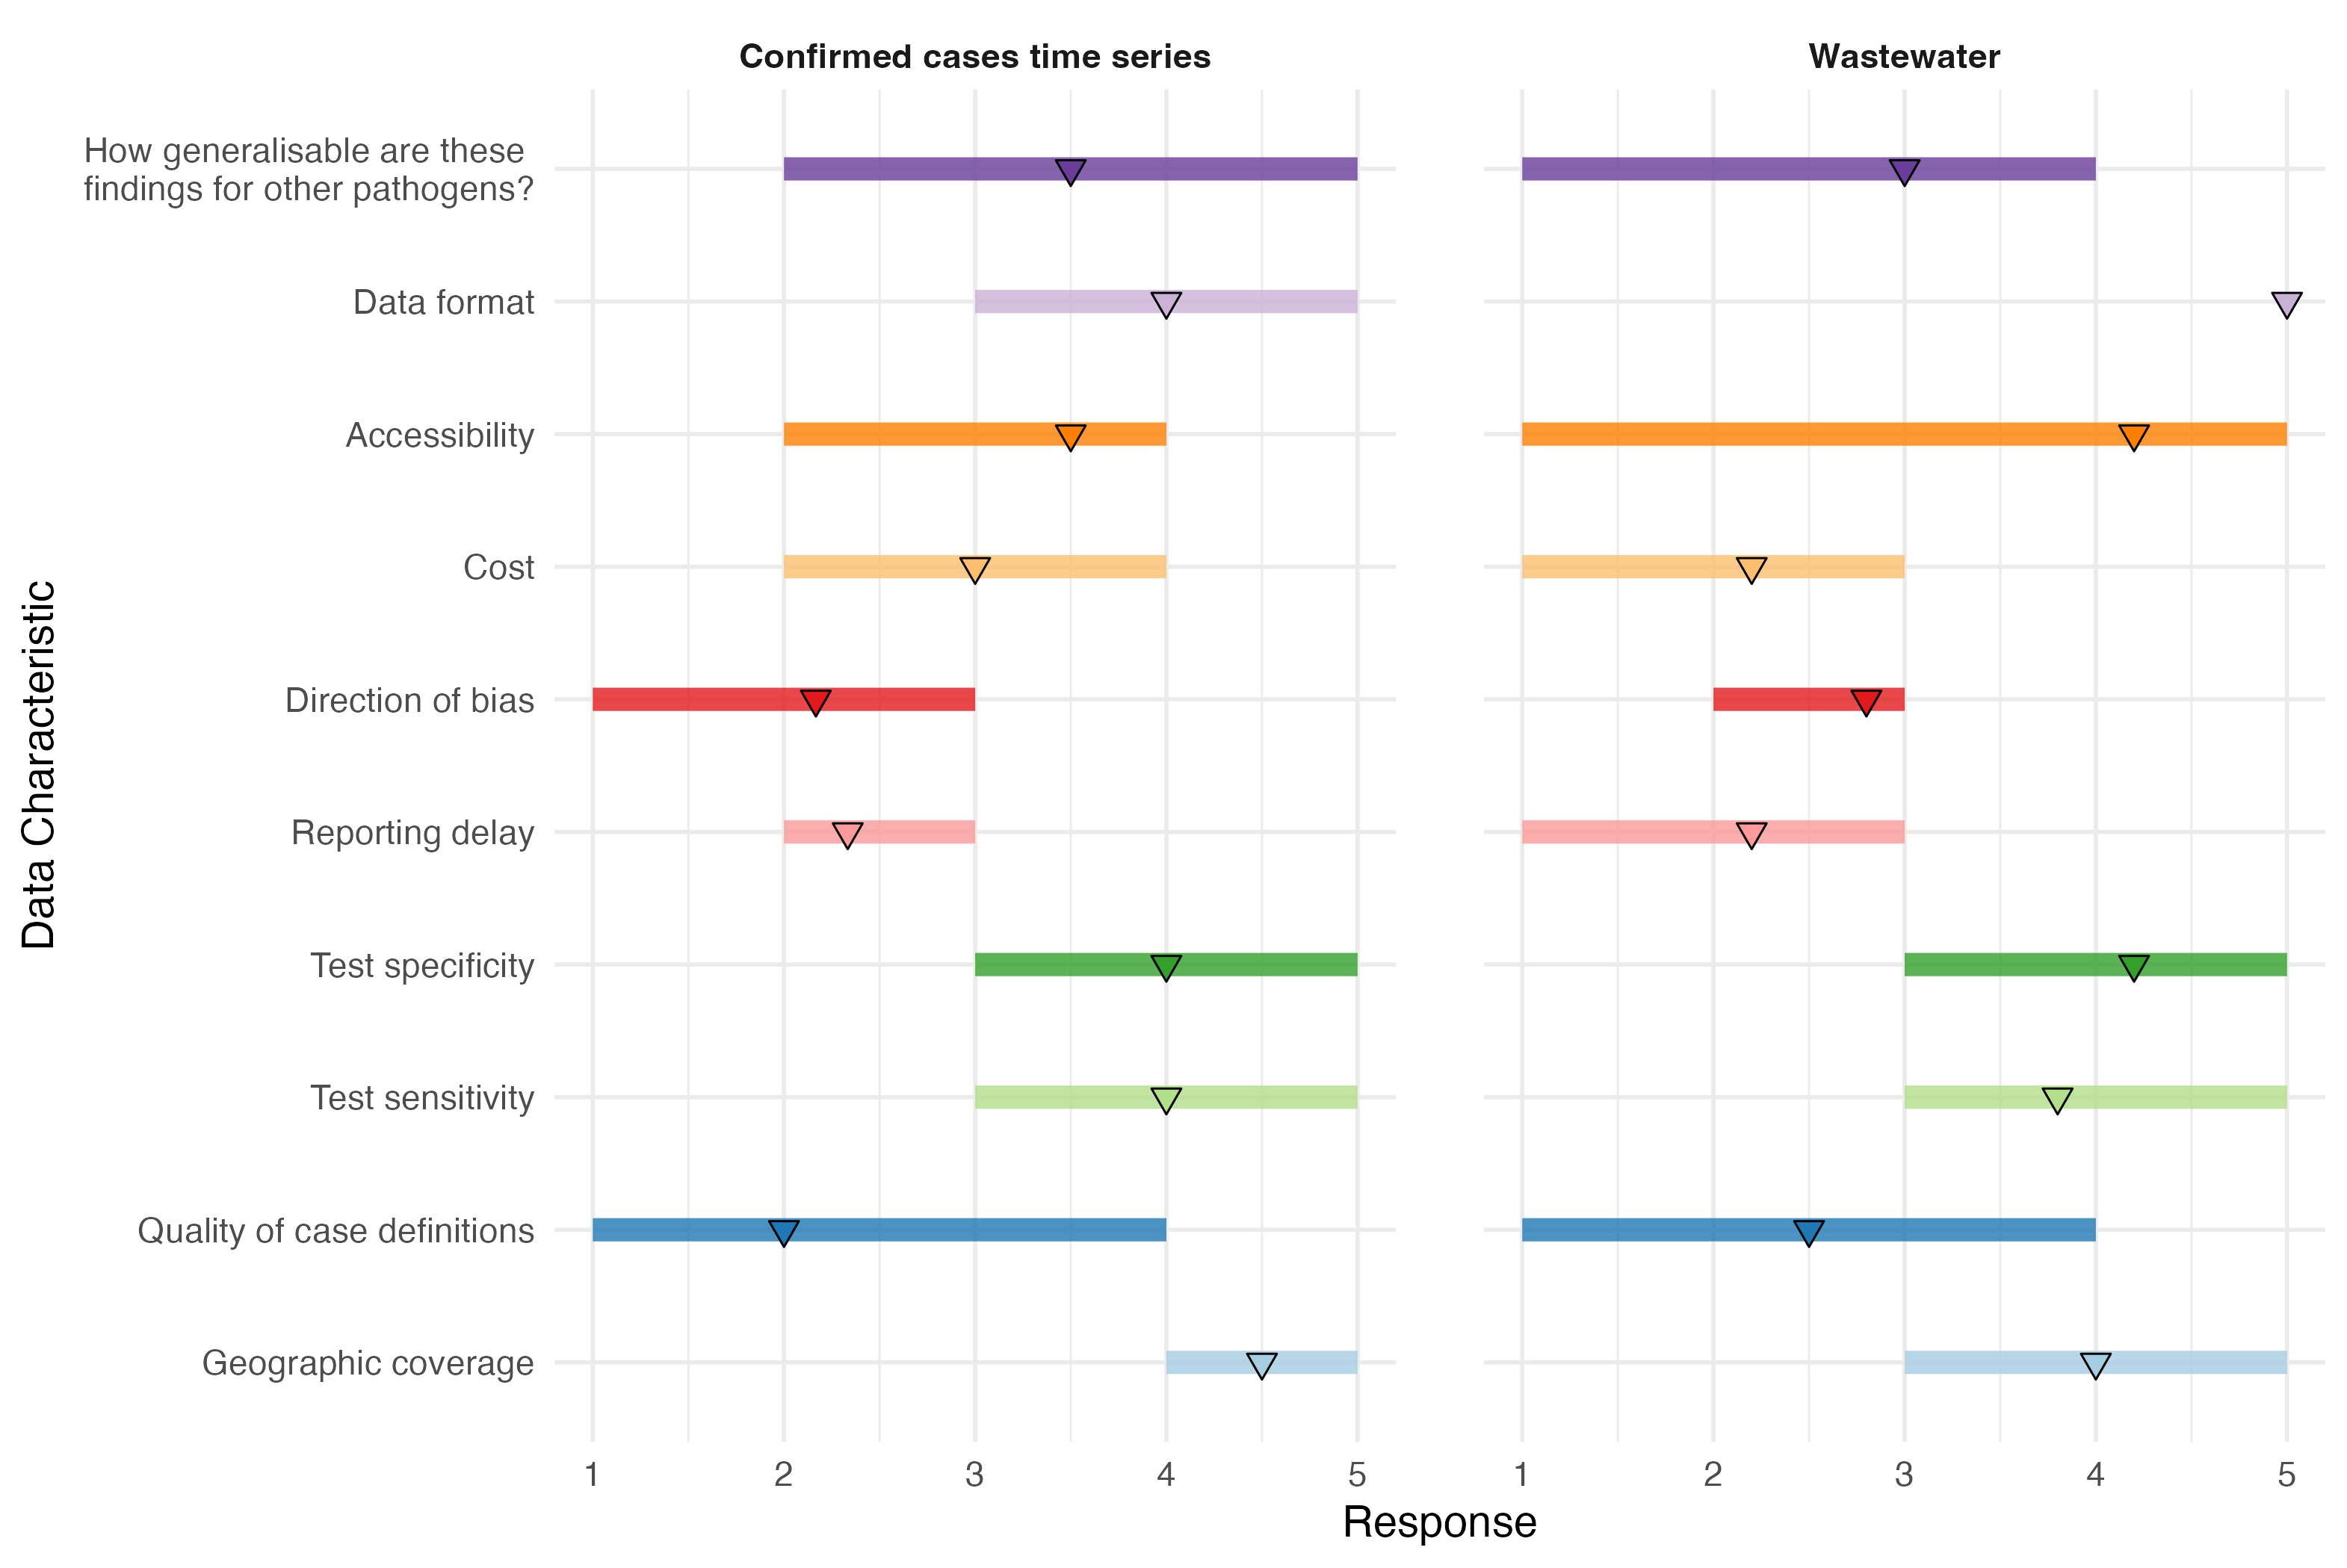
\includegraphics[width=.97\linewidth]{figures/survey_responses.png}
\centering
\caption{ Selected data characteristics from the survey, showing responses related to confirmed case time series (6 responses) and wastewater surveillance (5 responses). The y-axis represents specific data characteristics, while the x-axis indicates the response range on a 5-point scale, where 1 corresponds to a low level and 5 to a high level. The lower triangles present the average response for each data characteristic.}
\label{survey_responses}
\end{figure}

CALL BACK TO THE DATA SOURCES WORKFLOW PROPOSAL
SAY THIS IS A CASE STUDY OF DOING THIS

We made a big list across the authors using our approach. It was highly variable different views. useful to get it into text/data. See it in the SI

We then decided on a set of characteristics for the data sourves we consider in this case study. A focussed version of this is in table blah. As you can see blah blah blah
The full version of this is in SI. Interesting comment on free text

It is also useful to look in detail at individual data sources. Table blah is an example of this. Note blah and blah and blah.
We have the rest of these in the SI. 
The following case studies will demonstrate referring back to these and blah blah.



\subsection{Case Study 0: Single-Source Baseline (Cases Only)}


The research question for this case study (and case studies 1 and 2) is: what is the time-varying reproduction number $R_t$ during this outbreak period?
The objective of this case study is to showcase the workflow and explore some of the assumptions and modelling and fitting choices underlying estimation of $R_t$ from a single time series of case incidence.



\textbf{Workflow Demonstration:}
\begin{enumerate}
    \item \textbf{Process DAG development}: We consider three variants of the renewal process model for the number of new infections $I_t$ on day $t$, which is influenced by the reproduction number $R_t$ on day $t$, and the generation time (GT) distribution, which we assume to be fixed. The three model variants are:
\begin{itemize}
    \item[P1.] No variance in daily infection incidence (deterministic)
    \begin{equation} \label{eq:infections_P1}
        I_t = R_t \sum_{s=1}^\infty I_{t-s}w_s 
    \end{equation}
    \item[P2.] Poisson-distributed daily infection incidence.
        \begin{equation} \label{eq:infections_P2}
        I_t \sim \mathrm{Poiss}\left( R_t \sum_{s=1}^\infty I_{t-s}w_s  \right)
    \end{equation}
    \item[P3.] Negative binomially distributed daily infection incidence. 
            \begin{equation} \label{eq:infections_P3}
        I_t \sim \mathrm{NegBin}\left( R_t \sum_{s=1}^\infty I_{t-s}w_s, k  \right)
    \end{equation}
\end{itemize}
where $w_s$ is the probability mass function for the GT distribution and $k$ is the dispersion parameter. 
The process DAGs for these three models are shown in Figure \ref{fig:CS0_DAGs}.

 

\item \textbf{Data source mapping}: Case incidence data is typically readily available with very frequent updates and relatively good timeliness (good scope and resolution), though this can depend on lab processing and reporting timelines. However, it is an imperfect and potentially biased proxy for infection incidence, and is sensitive to testing patterns and the fraction of infections that are reported as cases (data quality issues). 


\item \textbf{Observation DAG construction}: The observation model relates the observed data (here daily case incidence) with underlying latent variables (here daily infection incidence). 
This requires assumptions to be made about underreporting (what fraction of infections are detected cases), reporting delays (time between infection and a case being detected and reported), and random noise (typically used to capture other things not explicitly specified in the model).

Alternative versions of the observation model can be considered, which either ignore or include each of these three aspects. This leads to $2^3=8$ possible observation models, each of which has an associated DAG (although some DAGs may be the same).
We refer to these models as $O_{000}$ (for the simplest observation model not modelling any of the above) to $O_{111}$ (for the most comprehensive accounting for all three observation features). 

The $O_{111}$ model could be represented by the following equation for the observed variable $\hat{I}_t$, representing the number of reported cases on day $t$:
\begin{equation}
    \hat{I}_t \sim \mathrm{Poiss}\left( \sum_{s=1}^t N_{s,t}\right)
\end{equation}
where $N_{s,t}$ is the number of people infected on day $s$ and reported as a case on day $t$, given by
\begin{equation}
    N_{s,t} \sim \mathrm{TruncatedMultinomial}\left( I_s, \alpha_{t-s}\right) 
\end{equation}
and $\alpha_j$ is the proportion of infections that are reported as a case $j$ days after infection ($j=0,1,\ldots$). 


\item \textbf{Data integration choices}: As there is only one data source in this case study, no decisions about what and how to integrate multiple sources are needed. The choice of fitting method may depend on considerations such as analytical tractability of the combined process and observation model, computational complexity and speed of computation relative to the time available, and identifiability issues. 
 
One scenario where integration would be required is model ensembling, where multiple estimates of the target estimand (in this case $R_t$) are produced by different groups or methods based on the same data, and synthesised into a combined estimate. [***Link to SPI-M paper from Oxford]. In this context, it may be desirable to align the assumptions made by different models, for example about the GT distribution or the temporal smoothness in $R_t$, to ensure that estimates from the different models are  comparable [***Johannes’ paper].

\item \textbf{Fitting choices}: Implementation requires selection of one process model, one observation model and one fitting and integration method (which will depend on the choice of process and observation model as described above). For this case study, combinations of the 3 process models and 8 observation models give 24 possible models, on top of which alternative fitting methods can be chosen for each. Here, we give a few examples from the literature:
\begin{itemize}
    \item EpiEstim. This method assumes Poisson distributed infections, no underreporting, no delays in reporting, and no observation noise \citep{cori2013new}. In our categorisation, this corresponds to process model P2 and observation model $O_{000}$. The model is fitted by calculating an analytic posterior distribution for $R_t$ from a conjugate prior, which is fast and computationally efficient. 
    \item EpiNow2 [***may need to specify a version]. This method assumes deterministic infection incidence with no underreporting, but with delays and random observation noise. In our categorisation, this corresponds $P_1-O_{011}$. This is fitted using XXX.
    \item Epidemia or EpiMap for NB process – TODO: check what they do!
\end{itemize}

Other possible choices of fitting methods that could be considered / why not (refer to relevant section in the overall framework description)
 \end{enumerate}
 
% TODO: add a Figure. This will be A visual of jigsaw puzzle presenting a library of P (process models), O (observation models) and F (fitting methods). In multi-data ones we will need to add an I (integration method) too.
% Example choices of EpiEstim and EpiNow2 for example (as above). Prototype figure below

% \begin{figure}
% 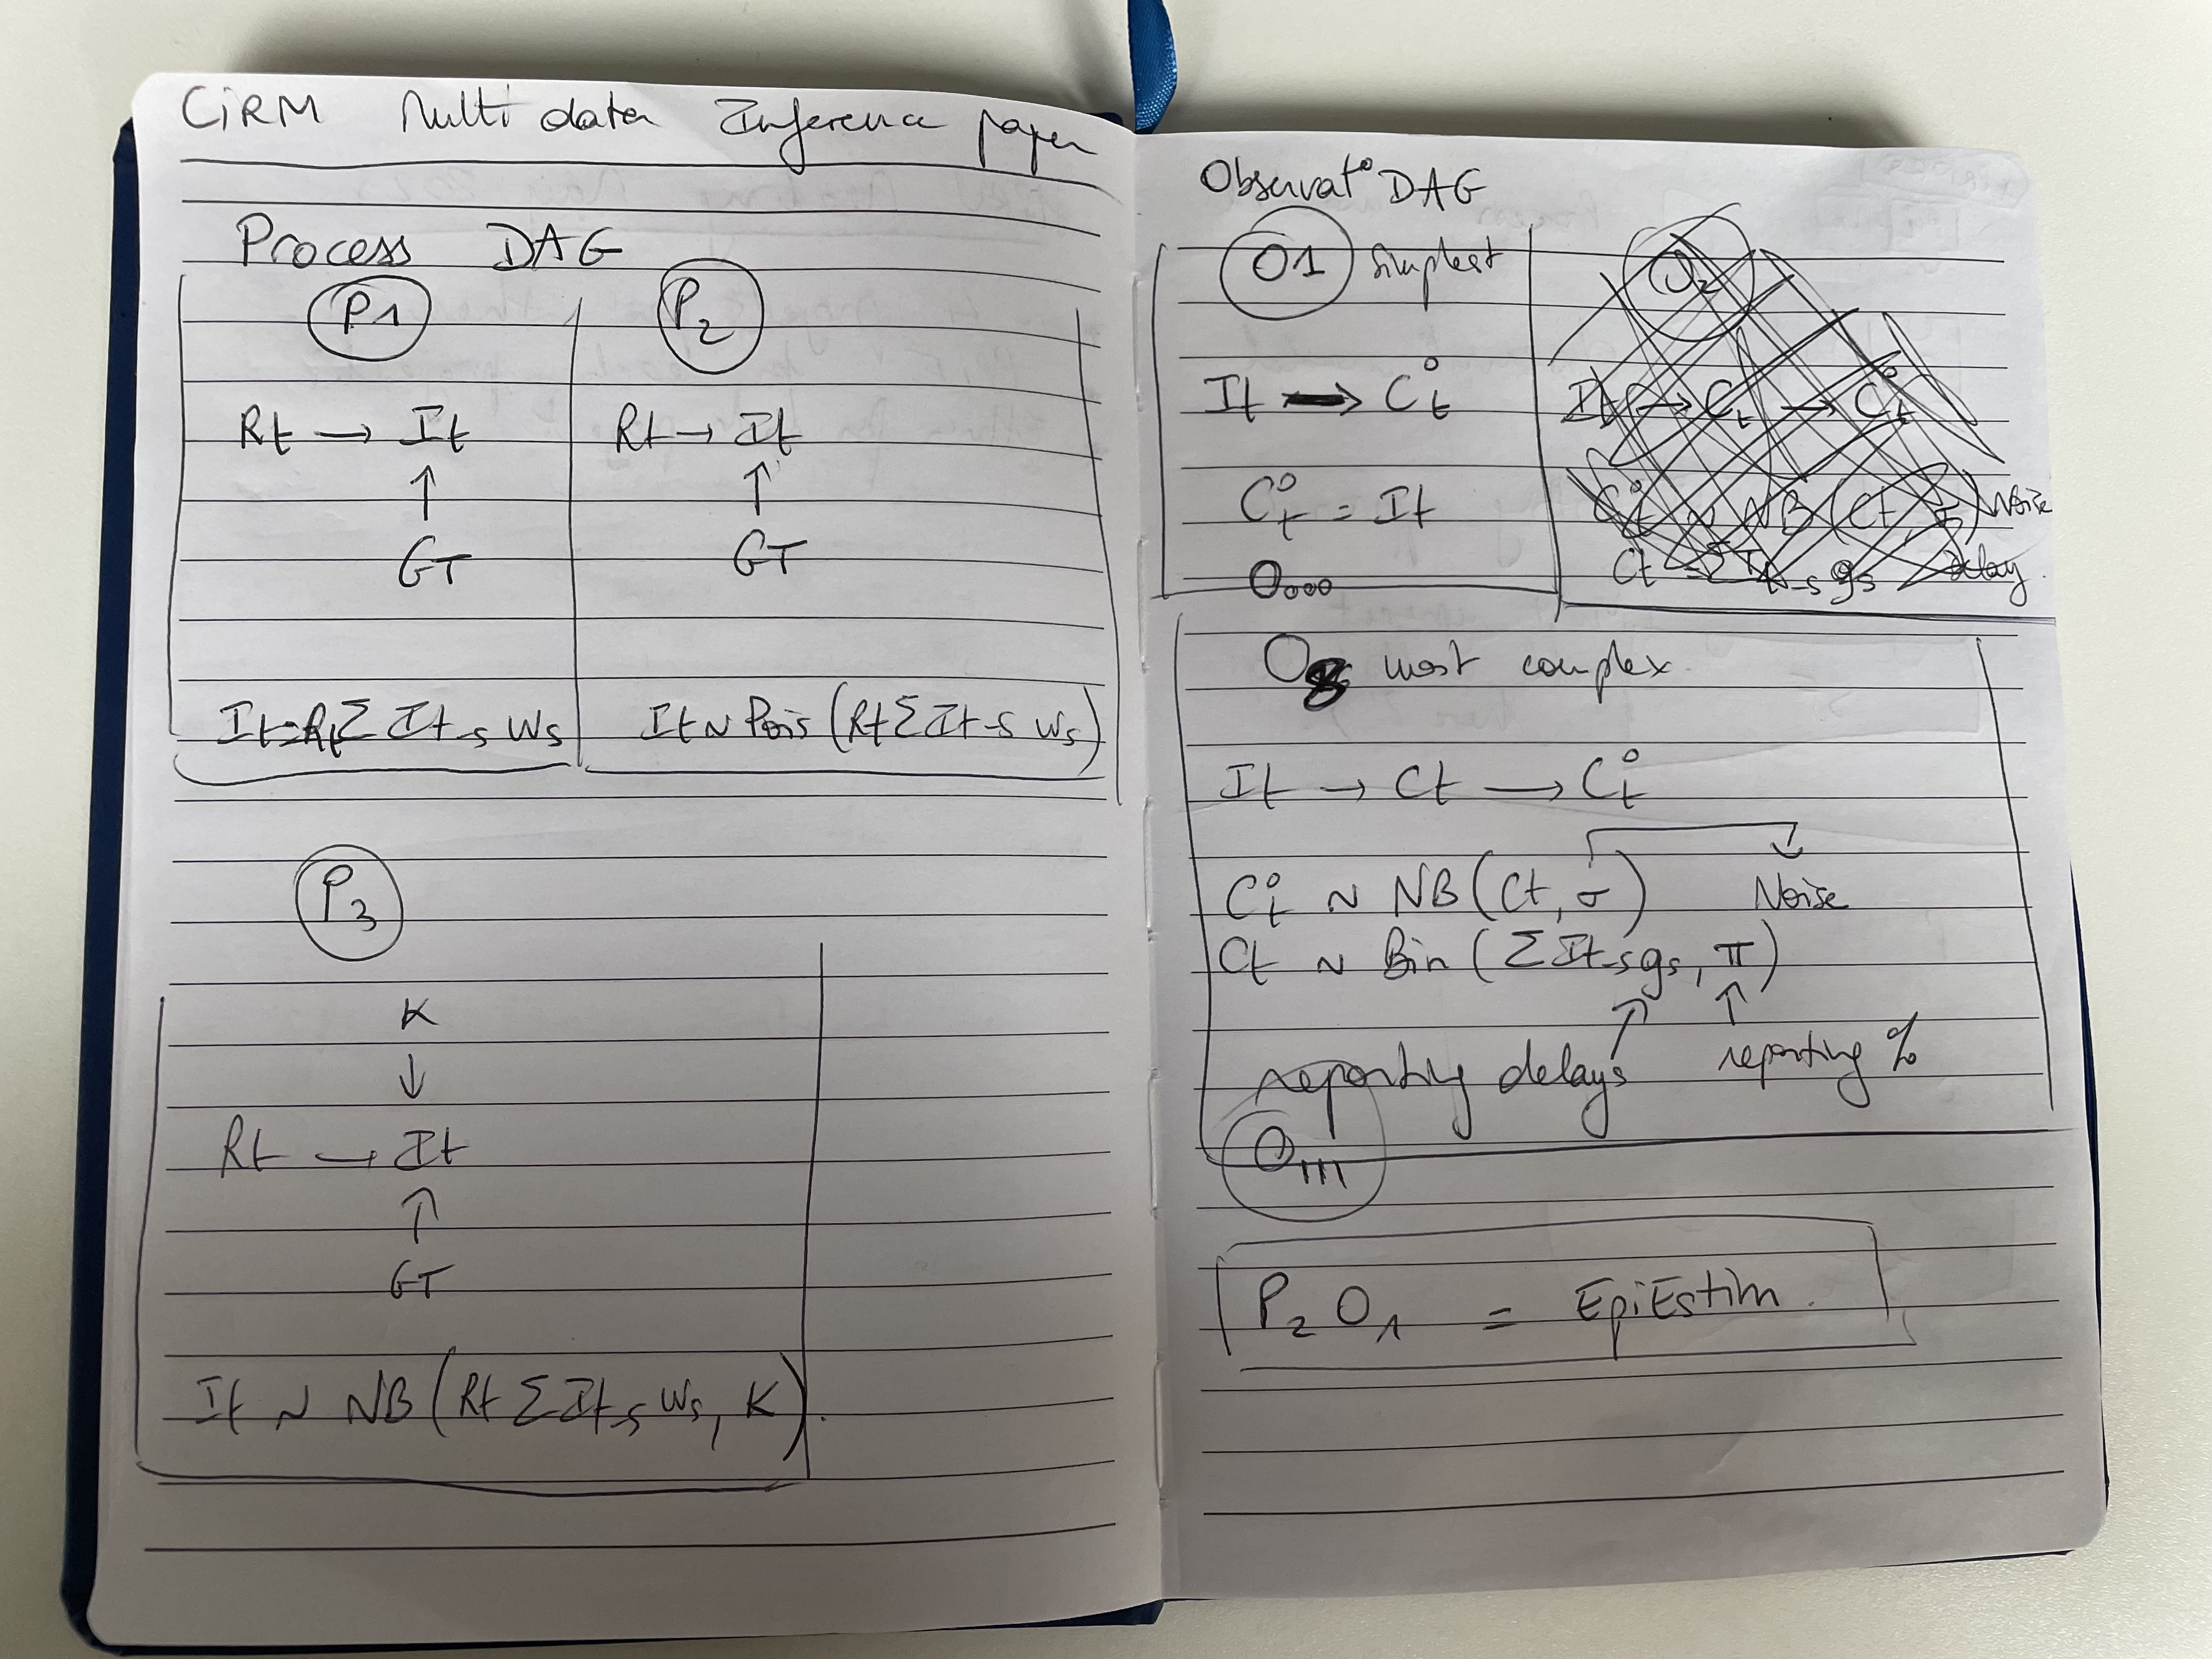
\includegraphics[width=0.75\textwidth]{figures/cs0_diagram1.jpg}
% \label{fig:CS0_DAGs}
% \caption{Process model DAGs for case study 0.}
% \end{figure}

% 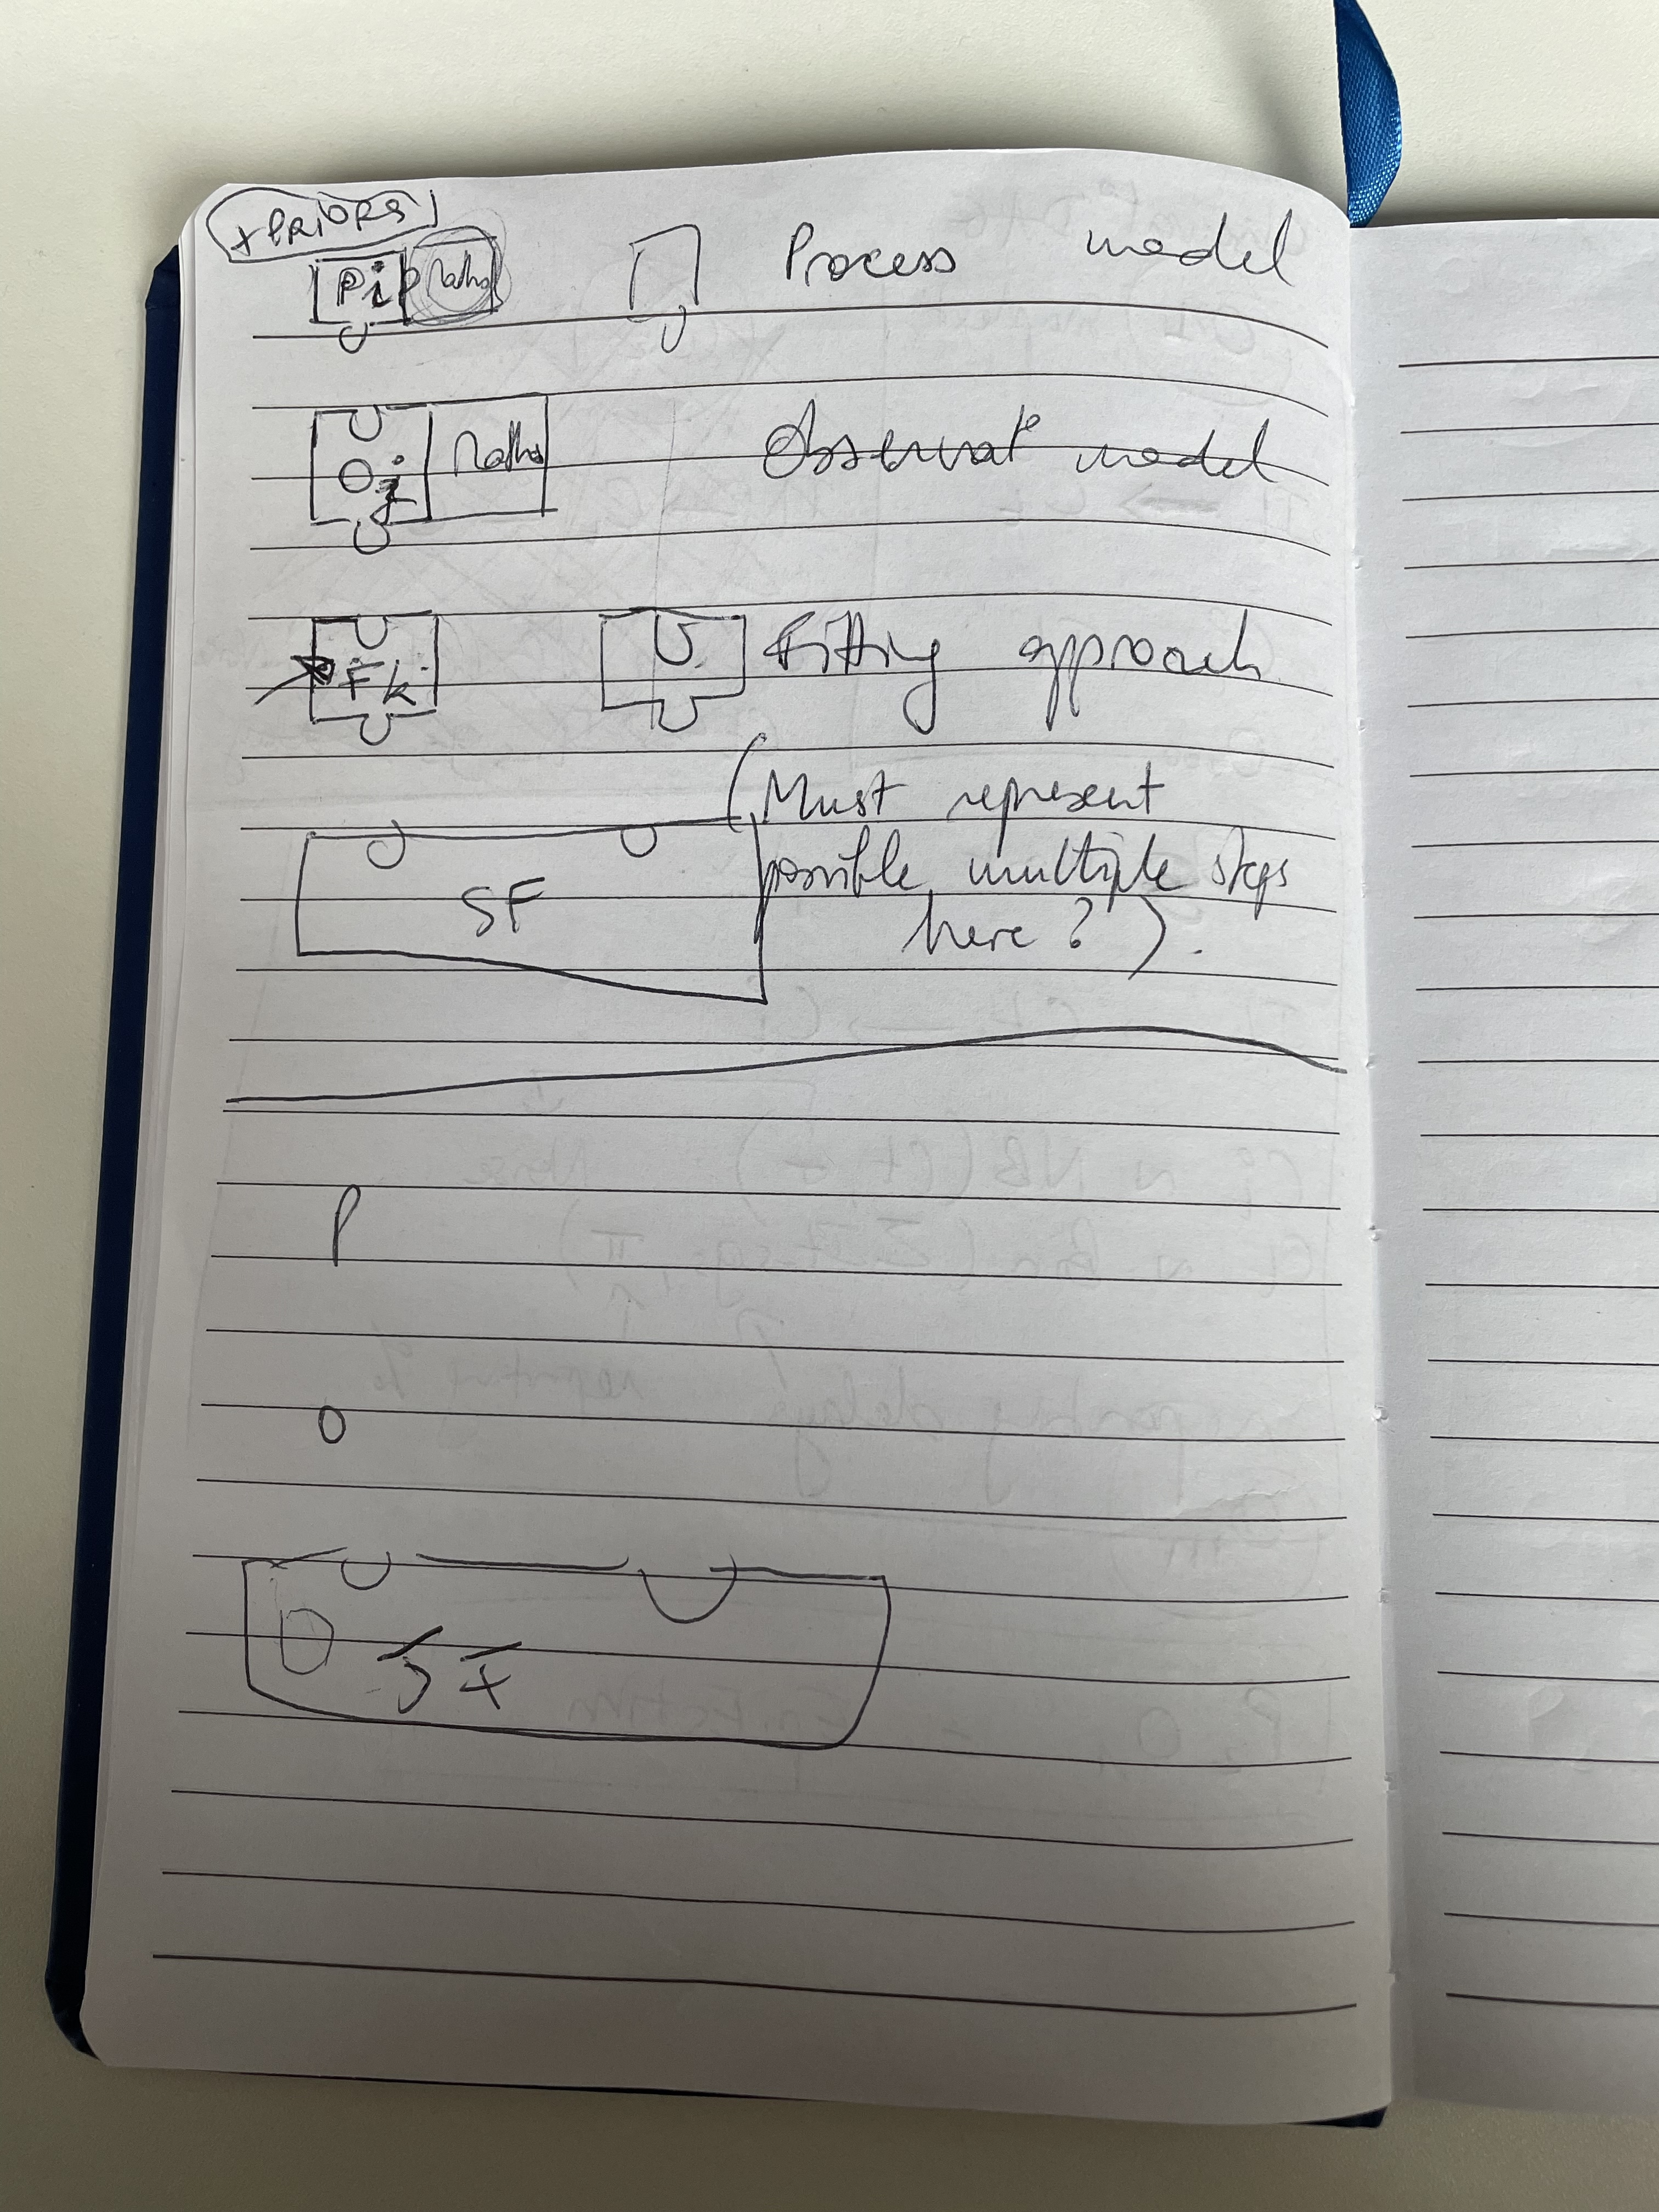
\includegraphics[width=0.75\textwidth]{figures/cs0_diagram2.jpg}

\begin{figure}[htbp]
    \centering
    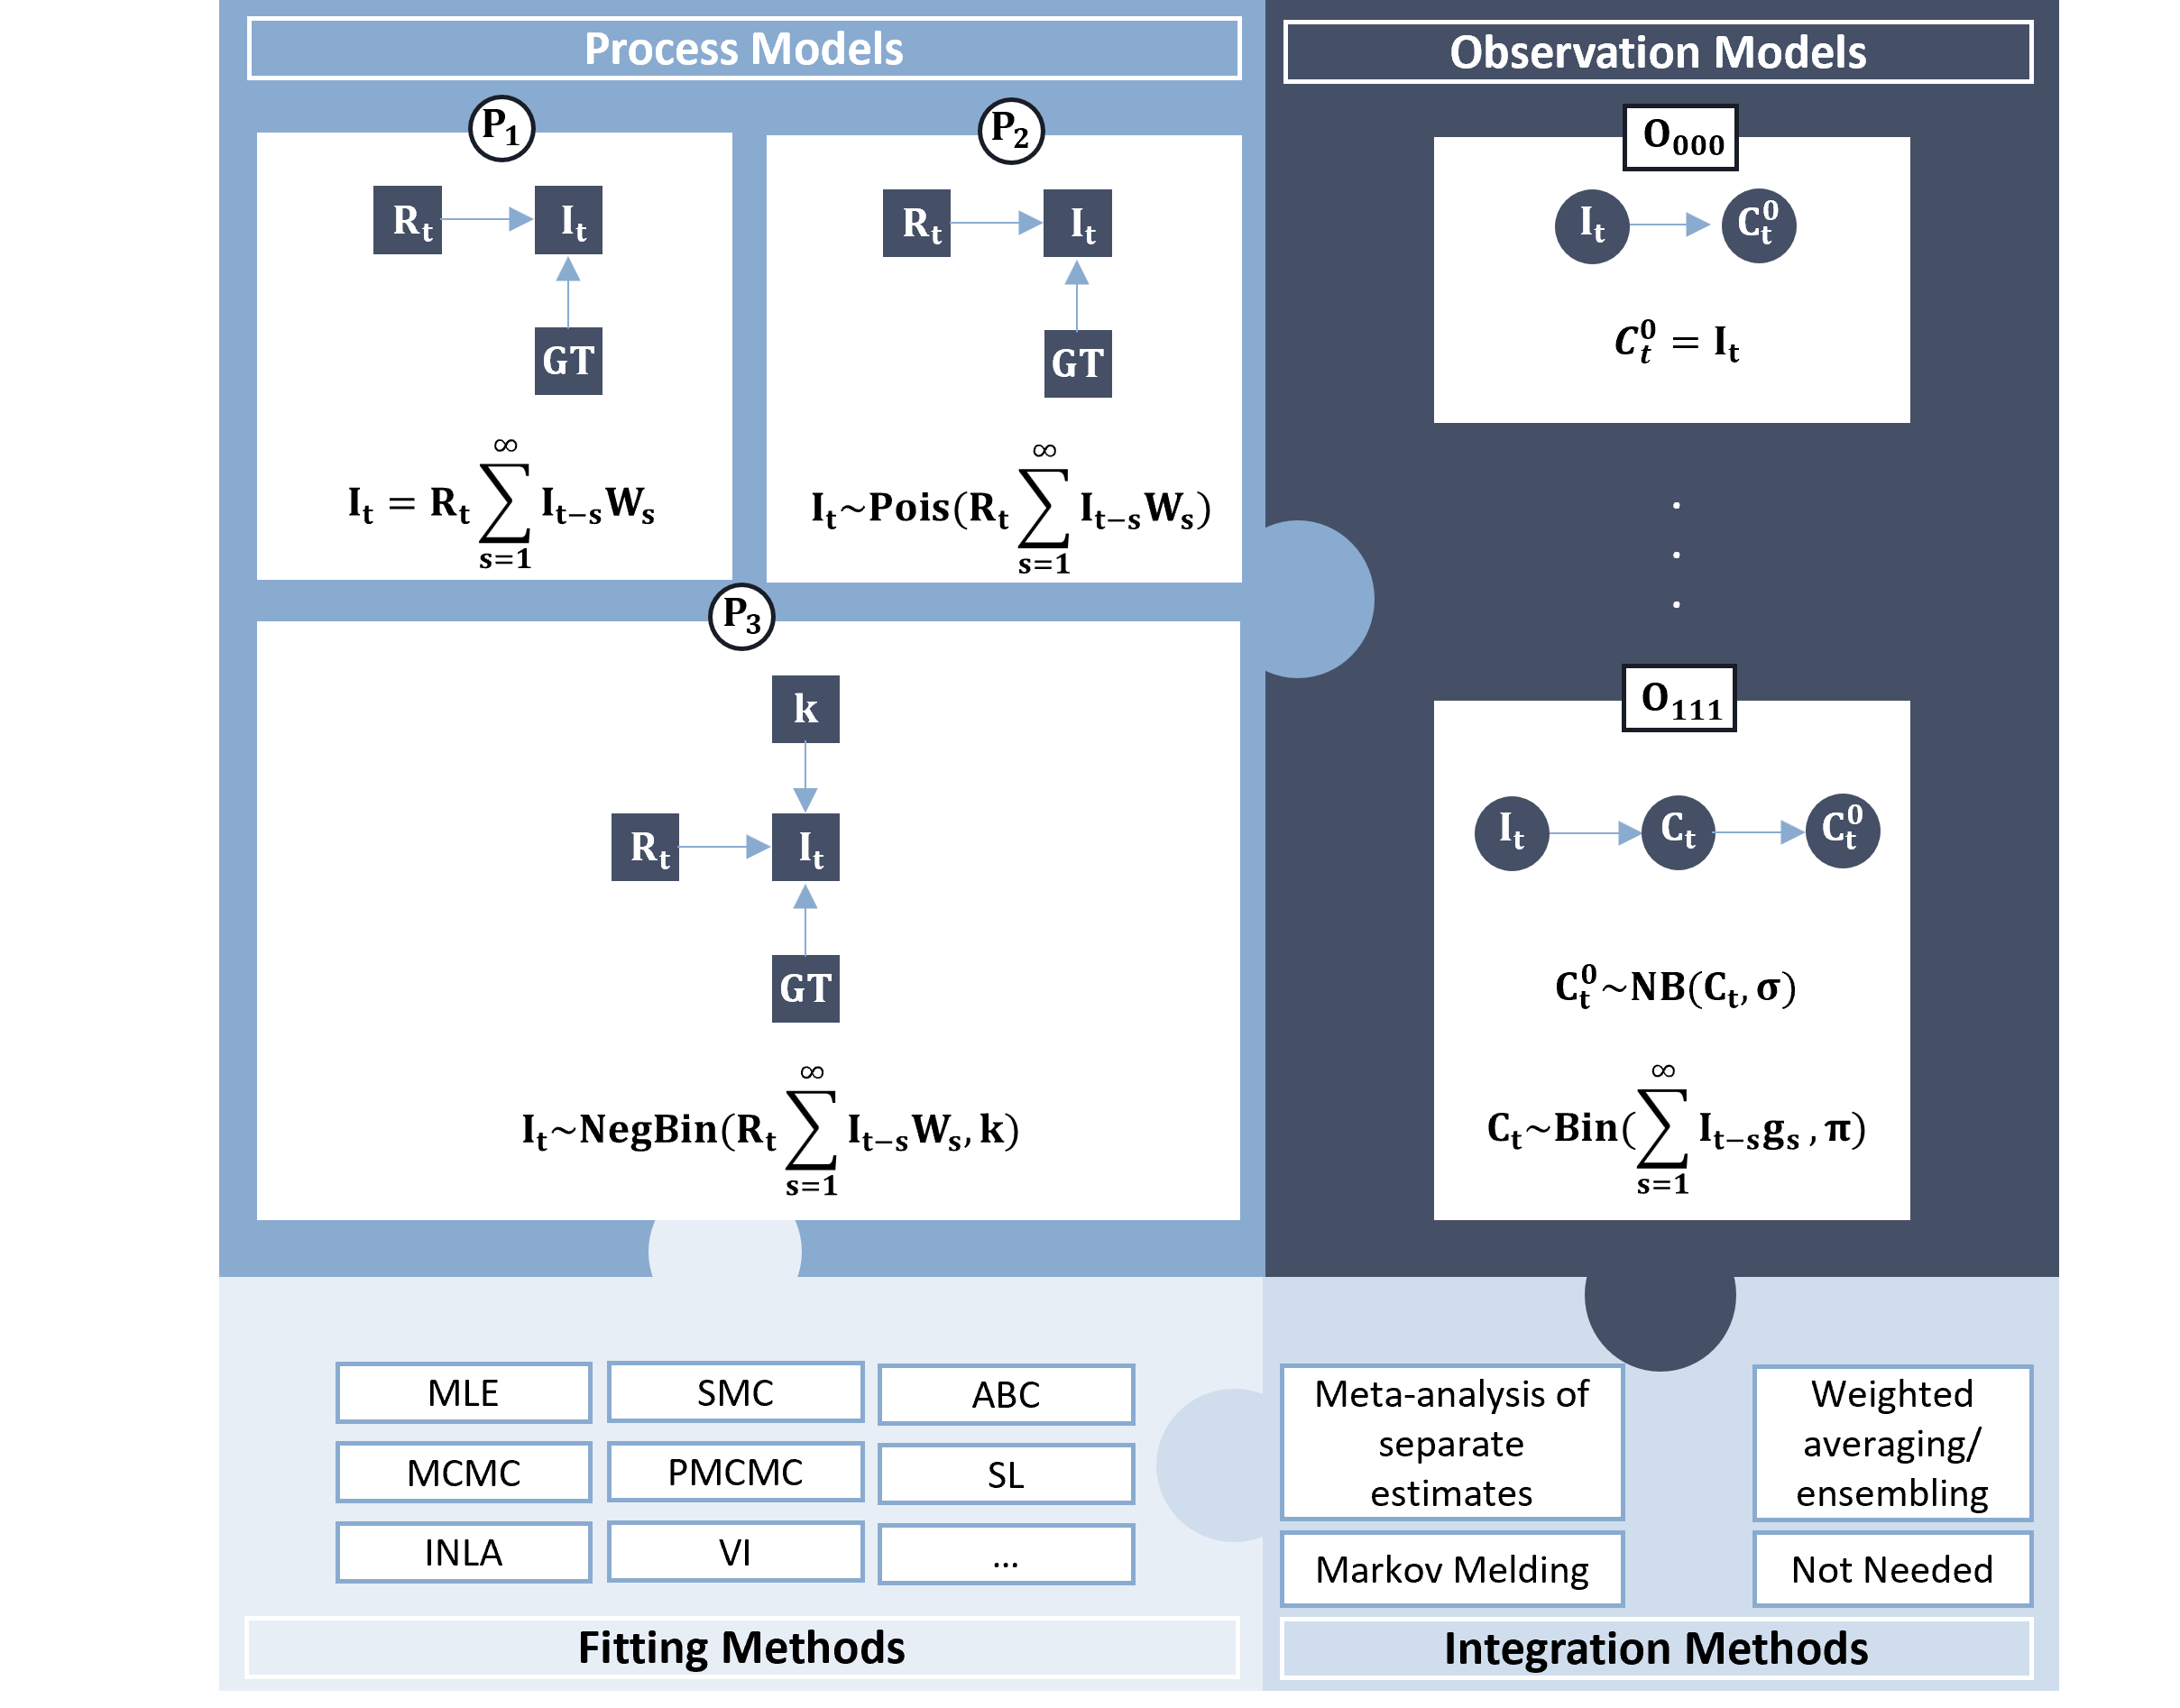
\includegraphics[width=\textwidth]{figures/case_study_jigsaw.png}
    \caption{\textbf{Modular representation for infectious disease modelling showing the interchangeable components of process models, observation models, integration approaches, and fitting methods.} Process models include deterministic ($P_1$), stochastic Poisson ($P_2$), and negative binomial ($P_3$) formulations relating reproduction number ($R_t$) to number of new infections ($I_t$) with generation time ($GT$) distributions. $P_3$ incorporates overdispersion parameter $k$ to caption extra-Poisson variation. Observation models range from direct observation ($O_{000}$) to complex hierarchical structures ($O_{111}$) that model the relationship between $I_t$ and (observed) case incidence ($C_t$) through reporting delays and measurement uncertainty. Integration approaches span from meta-analysis of separate estimates to weighted averaging approaches, enabling researchers to select optimal combinations based on data availability and research objectives. The jigsaw puzzle metaphor illustrates how different modelling components can be combined flexibly, with fitting method including MCMC, VI, ABC, etc.}
    \label{fig:case_study_visual}
\end{figure}



Different approaches have different strengths and limitations. For example, the key strength of EpiEstim is computational speed, whereas its key weaknesses are ignoring underreporting and reporting delays. The former may be less important in contexts where the reporting fraction can reasonably be assumed to be steady over the time period of interest. Furthermore, any change in reporting fraction will not be identifiable from a case time series alone, so it would not be sensible to attempt to estimate this in this example. EpiNow2 overcomes some of these weaknesses, at the cost of increased computational complexity. The more appropriate option may depend on the balance between need for timely estimates (e.g. for modelling an outbreak in real-time) and the realism of the associated assumptions. 

A common weakness of all the models outlined above is that they assume the GT distribution is constant and perfectly known. Some approaches (e.g. some versions of EpiEstim) extend the approach to relax this assumption (see also Case Study 4).
 



\subsection{Case Study 1: Two-Source Integration (Cases and Deaths)}

The target estimand for this case study is the same as in case study 0 ($R_t$). The objective of this case study is to illustrate the process and challenges of adding an additional data stream (in this case death data), and to explore how this can improve $R_t$ estimation and reduce assumption dependence.

\textbf{Workflow Demonstration:}
\begin{enumerate}
    \item \textbf{Process DAG development:} The number of deaths $D_t$ on day $t$ depends on the time series of infections up to day $t$, the infection-fatality ratio $p_d$, and the distribution $v_s$ of time ($s$) from infection to death. This can be represented in the process DAG (Figure \ref{fig:CS3_DAG}a) and by the following convolution equation:
    \begin{equation} \label{eq:deaths}
        D_t \sim \mathrm{Poiss}\left(p_d \sum_{s=1}^\infty I_{t-s}v_s \right)
    \end{equation}
    Other process models for deaths are possible, for example using a multinomial model for the number of deaths occurring on day $s+k$ due to infections on day $s$ ($k=1,2,\ldots$). However, the Poisson model is a good approximation provided $p_d\ll 1$. This formulation assumes that the probability $p_d$ of an infection resulting in death and the distribution of time from infection to death $v_s$ are fixed and known.
    
    Eq. \eqref{eq:deaths} provides a model for the time series of daily deaths $D_t$ conditional on the time series of daily infections $I_t$ and would typically be used in combination with one of Eqs. \eqref{eq:infections_P1}--\eqref{eq:infections_P3} that describe the dynamics of infections to produce a joint model for infections and deaths. 
    \item \textbf{Data source mapping:} Data on deaths typically have longer delays (delay from infection to death and potentially from date of death to date of registration), but lower noise (e.g. due to ``day-of-the-week'' reporting effects), higher ascertainment, and less dependence on testing patterns than case incidence data. Combining deaths data with cases therefore has the potential to overcome some of the limitations present in each single data source. 
    \item \textbf{Observation DAG construction:} Similar to the different choices of observation model for cases described in case study 0 (and still relevant to this case study), the observation model for deaths could include underreporting, reporting delays, and random noise. In jurisdictions with comprehensive death records, it may be reasonable to assume all deaths are reported and there is no additional observation noise, but it may still be important to account for observation delays, for example delay from date of occurrence to date of registration \citep{seaman2022nowcasting}. 
    This would corresponds to observation model $O_{010}$, with the following equation for observed variable $\hat{D}_t$, representing the number of deaths registered on day $t$:
\begin{equation}
    \hat{D}_t = \sum_{s=0}^\infty M_{s,t}
\end{equation}
where $M_{s,t}$ is the number of deaths that occurred on day $s$ and were registered on day $t$, given by
\begin{equation}
    M_{s,t} \sim \mathrm{Multinomial}\left( D_s, \beta_{t-s}\right) 
\end{equation}
and $\beta_s$ is the probability mass function for the number of days from date of death to date of registration ($s=0,1,\ldots$).
    
    \item \textbf{Data integration choice:} 
       Two different approaches are possible for integration: (1) a joint model including both cases and deaths with a shared latent state $R_t$; (2) separate models for cases and deaths, resulting in two estimates for $R_t$ to be combined via a weighted ensemble. 
       
       As outlined above, we recommend fitting separate models to the two time series initially, to understand their behaviour and reveal whether they lead to consistent or conflicting estimates of $R_t$. Where inconsistent results emerge, these could lead to refinement of the model (i.e. going back to step 1). For example, if $R_t$ estimates show similar trends but shifted in time, assumptions about delays may be revisited. If $R_t$ estimates are largely consistent, but the case-based estimate shows a transient increase in $R_t$ that does not occur in the deaths-based estimate, this could indicate a change in case ascertainment, which may require refining the model. Once this has been done, it may be desirable to combine the results into a single estimate by ensembling, or to fit a joint model that produces a single estimate from both data sources.  
       
    \item \textbf{Fitting choices:} For separate models, a good choice would be NUTS for estimation, followed by Markov melding to ensemble the results from the two models. For a joint model, a numerical method such as particle MCMC would likely be needed due to the state-space formulation complexity.

    \textcolor{red}{I think we should add some examples from the literature here. Just adding some notes for now:} 1) EpiNow2 seems to allow fitting jointly to cases and deaths: \url{https://wellcomeopenresearch.org/articles/5-112} - they use P1 for infections, but not very clear about cases and deaths - would need Sam's help here 2) this has several models based just on deaths - the last one uses cases and deaths but I don't think has a mechanisms for cases changing over time \url{https://journals.plos.org/plosone/article?id=10.1371/journal.pone.0286199} 3) I think Epidemic uses only deaths actually \url{https://static-content.springer.com/esm/art%3A10.1038%2Fs41586-020-2405-7/MediaObjects/41586_2020_2405_MOESM1_ESM.pdf}

    \end{enumerate}

\textbf{Key Insight:} In case study 0 using data on cases alone, the case ascertainment rate (i.e. the proportion of infections that are reported as cases) was non-identifiable and had to be assumed. Including data on deaths, if the infection-fatality ratio is known, means that the case ascertainment rate could be included as a target for estimation. However, this requires assumptions about the distribution of time from infection to death, demonstrating how additional data sources can shift rather than eliminate the need for modelling assumptions.

\subsection{Case Study 2: Three-Source Integration (Cases, Deaths and Wastewater)}

The target estimand for this case study is the same as in the previous case studies ($R_t$). The objective of this case study is to explore ways of handling conflicting signals between data sources and incorporating complex observation processes.

\textbf{Workflow Demonstration:}
\begin{enumerate}
    \item \textbf{Process DAG development:} 
    Suppose that the average concentration $W_t$ of pathogen RNA/DNA in wastewater on day $t$ depends on the time series of infections up to day $t$ and the average amount of pathogen RNA/DNA that an individual sheds into wastewater $s$ days after being infected ($s=1,2,\ldots$). This can be represented in the process DAG (Figure \ref{fig:CS3_DAG}a) and by the following equation for $W_t$:
    \begin{equation} \label{eq:wastewater}
        W_t \sim \Gamma\left( \frac{C}{N_\mathrm{pop}}\sum_{s=1}^\infty I_{t-s}u_s, b   \right)
    \end{equation}
    where $C>0$ is a constant representing the average total amount of pathogen RNA/DNA that an infected individual sheds over the course of their infection, $N_\mathrm{pop}$ is the population size, $u_s$ is the average shedding rate $s$ days after infection normalised such that $\sum_{s=1}^\infty u_s=1$, and $\Gamma(\mu,b)$ denotes a gamma distribution with mean $\mu$ and shape $b$. This was similar to the wastewater model used by \cite{watson2024jointly}; other choices of continuous non-negative-valued distributions are possible for $W_t$ such as a log-normal distribution.

    Eq. \eqref{eq:wastewater} would be combined with one of Eqs. \eqref{eq:infections_P1}--\eqref{eq:infections_P3} for infections and with Eq. \eqref{eq:deaths} for deaths.
    \item \textbf{Data source mapping:} Wastewater data offers population-level information (broad scope) independent of testing biases and changes in testing rates, with moderate timeliness, requiring environmental expertise and subject to high levels of unexplained variability. It could also be affected by unknown changes in the average shedding rate $C$ over time and has relatively poor resolution (limited spatial resolution and no information about age or other demographic variables). 
    \item \textbf{Observation DAG construction:} 
   Wastewater samples are typically collected at some cadence from one or more sampling sites, and the concentration of pathogen RNA in the samples is quantified via PCR testing. 
   The existence of multiple sites with different catchments populations and non-contemporaneous sampling frequencies complicates the interpretation of quantitative wastewater data, which can be modelled at varying levels of complexity.  
   
    Here, we assume that a noise-free measurement of the wastewater concentration $W_t$, either from a single representative site or a suitable average of multiple sites, is taken on some subset of days $t$. Then the equation for the observed variable $\hat{W}_t$ is simply
    \begin{equation}
        \hat{W}_t=W_t
    \end{equation}
    If required, observation noise could be included by replacing this with a distribution with mean $W_t$. 
    More complex models could also incorporate other factors such as individual-level and site-level variation, catchment population dynamics, spatial heterogeneity, different sampling methods, and environmental degradation.
    \item \textbf{Data integration choice:} As in case study 1, we recommend that a modular approach with sequential consistency assessment is initially taken to detect and resolve data source conflicts. For example, a time lag in estimates of $R_t$ from wastewater data alone relative to estimates of $R_t$ from cases alone could suggest misspecification of the shedding rate distribution $u_s$. Once conflicts have been identified and resolved, independent estimates of $R_t$ from these models could be combined by ensembling, or a joint model could be fitted with a shared $R_t$ state. 
    \item \textbf{Fitting choices:} ABC-SMC for wastewater sub-model due to likelihood intractability, reflecting available environmental modelling expertise; NUTS for case/death models. For a joint model, a method like particle MCMC would likely be needed due to the state-space complexity.
\end{enumerate}

\textbf{Key insight:} Wastewater data enables trend estimation independent of shifts in testing patterns, but requires assumptions about the shedding, environmental and sampling processes. A modular approach facilitates conflict detection between data sources. The average shedding rate $C$ is typically unknown and non-identifiable from available data. Similar to the unknown case ascertainment rate in case study 0, estimates of $R_t$ will be insensitive to the value of $C$ provided it does not change over time. However, changes in the average shedding rate due to, for example, pathogenic evolution or changes in population immunity, would invalidate this simple model and require a more nuanced approach.  



\subsection{Case Study 3: Individual-Level Data (Cases and Transmission Pairs)}

The research question for this case study is what is the time-varying reproduction number $R_t$ and how much heterogeneity is there in individual transmission rates? The latter is captured by the additional estimand $k$, representing the dispersion in the distribution of the number of secondary cases per index case. The objective of this case study is to illustrate how different types of data (time series count data and individual-level data from contact tracing records) can be combined to enable estimation of additional quantities. 


\textbf{Workflow Demonstration:}
\begin{enumerate}
    \item \textbf{Process DAG development:} Including information on individual-level variables, as opposed to just aggregate daily counts, requires a shift from the population-level renewal equation (Eqs. \eqref{eq:infections_P1}--\eqref{eq:infections_P3}) to an individual-level model which explicitly represents the transmission tree. A DAG for this type of model is shown in Figure \ref{fig:CS3_DAG}. Mathematically, this can be expressed in terms of the number $N_{i,t}$ of people newly infected by individual $i$ on day $t$:
    \begin{equation} \label{eq:individual_level}
    N_{i,t} \sim \mathrm{Poiss} \left( Y_i R_t w_{t-T_i} \right)
    \end{equation}
    where $T_i$ is the infection time of individual $i$ and $Y_i$ is a continuous, non-negative random variable with mean $1$, representing the relative transmission rate of individual $i$ (which may capture a combination of biological and social factors). This formulation provides a way to explicitly simulate the full epidemic transmission tree.  In the special case where $Var(Y)=0$ (i.e. there is no individual-level heterogeneity), the total number of new infections on day $t$ ($I_t$) reduces to Eq. \eqref{eq:infections_P2}. 
    %For a case with given values of $Y_i$ and $T_i$, the total number of secondary cases, $Z_i=\sum_t N_{i,t}$, is
    %\begin{equation}
    %   Z_i \ | \ (Y_i, T_i) \sim \mathrm{Poiss}\left( Y_i \tilde{R}_{T_i}\right)
    %\end{equation}
    %where $\tilde{R}_t= \sum_s R_{t+s} w_s$ is the effective reproduction number averaged over the infectious period of an individual who was infected on day $t$. 
    If $Y\sim \Gamma(1,k)$ for some dispersion parameter $k$, then the number of secondary cases caused by an individual who was infetced at a given time $T_i=t$ is \citep{lloyd2005superspreading}
     \begin{equation} \label{eq:offspring_dist}
        Z_i \ | \ (T_i=t) \sim \mathrm{NegBin}\left( \tilde{R}_{t}, k\right)
    \end{equation}   
    where $\tilde{R}_t= \sum_s R_{t+s} w_s$ is the effective reproduction number averaged over the infectious period of an individual who was infected on day $t$.
    Note that this model assumes that the relative infectiousness profile over time $w_s$ is fixed and identical for all individuals. This is a reasonable starting assumption, but it may be important to relax this in some situations, for example to model the impact of quarantine and isolation measures on individuals identified by contact tracing.
    \item \textbf{Data source mapping:} Case studies 0, 1 and 2 only consider aggregate-level data on daily counts or wastewater measurements. This type of data typically only allows estimation of average transmission, i.e. $R_t$. In contrast, contact tracing records identify transmission pairs, which contain information about heterogeneity in transmission patterns, contingent on contact tracing system quality. The smaller the dispersion parameter $k$, the more variance would be expected in the distribution of the number of secondary infections per index case.
    \item \textbf{Observation DAG construction:} Suppose that for some subset of reported cases $i$, the number of observed secondary cases $\hat{Z}_i$ associated with that index case is recorded. For simplicity, we assume that the index cases for whom this data is available are a randomly chosen subset of all reported cases, and each secondary infection independently has fixed probability $p_l$ of being linked to the index case. We assume that all linked secondary cases are associated with the correct index case (i.e. we ignore any misclassification and uncertainty about who infected whom). 

   Then the probability that an index case reported on day $\tau_i$ has $\hat{Z}_i$ linked secondary cases can be calculated by conditioning on the unobserved time of infection $T_i$:
   \begin{equation}
       P(\hat{Z}_i=z \ | \ \tau_i=t) = \sum_{s=1}^{t} F_{NB}(z; p_l\tilde{R}_s,k) P(T_i=s | \tau_i=t)
   \end{equation}
where $F_{NB}(.;\mu,k)$ is the probability mass function for a negative binomial distribution with mean $\mu$ and dispersion $k$, and $R_i$ is the reporting time for case $i$.  The conditional probability in this equation can be calculated via Bayes' theorem to give
   \begin{equation} \label{eq:Zhat}
       P(\hat{Z}_i=z \ | \ \tau_i=t) = \frac{\sum_{s=1}^{t} F_{NB}(z; p_l\tilde{R}_s,k) \alpha_{t-s} I_s}{\sum_{s=1}^{t}\alpha_{t-s} I_s}  
   \end{equation}
 where $\alpha_j$ is the proportion of infections that are reported as a case $j$ days after infection ($j=0,1,\ldots$).
    % If we ignore delay from infection to reporting (i.e. observation model $O_{101}$ for infections) then the observed values of $\hat{Z}_i$ for cases reported on day $t$ are independent draws from
    % \begin{equation} \label{eq:Zhat}
    % \hat{Z}_i \sim \mathrm{NegBin}\left(p_l \tilde{R}_t, k\right)
    % \end{equation}
    % In practice, it would usually be important to account for delays from infection to observation (i.e. observation model $O_{111}$ for infections). This would complicate the model considerably as it requires knowledge of the distribution of time of infection conditional of time of report (which is not the same as the distribution of time of report conditional on time of infection, and in general will depend on the reproduction number $R_t$).
    % \item \textbf{Data integration choices:} A hierarchical model linking individual transmission events to population-level reproduction number would be a suitable framework.
    \item \textbf{Fitting choices:} NUTS with data augmentation for unobserved transmissions, chosen for efficient handling of discrete latent variables. Alternative a method such as particle marginal Metropolis Hastings could be used to used to estimate the time-varying reproduction number $R_t$ and the fixed parameter $k$ in a hierarchical manner (but may be computationally slow). 
\end{enumerate}

\textbf{Key Insight:} Individual-level data enables direct overdispersion estimation without distributional assumptions but requires contact tracing completeness assumptions. This shows how data granularity can fundamentally change model structure and inference requirements. However, it should be noted that the observed variable $\hat{Z}_i$ in Eq. \eqref{eq:Zhat} may not be available in real time as information about linked secondary cases will take time to collect. Furthermore, the distribution of  $\hat{Z}_i$ depends on future values of the latent variable $R_t$ and this means the model is not suitable for real-time inference. 

\begin{figure}
\centering
(a) \\
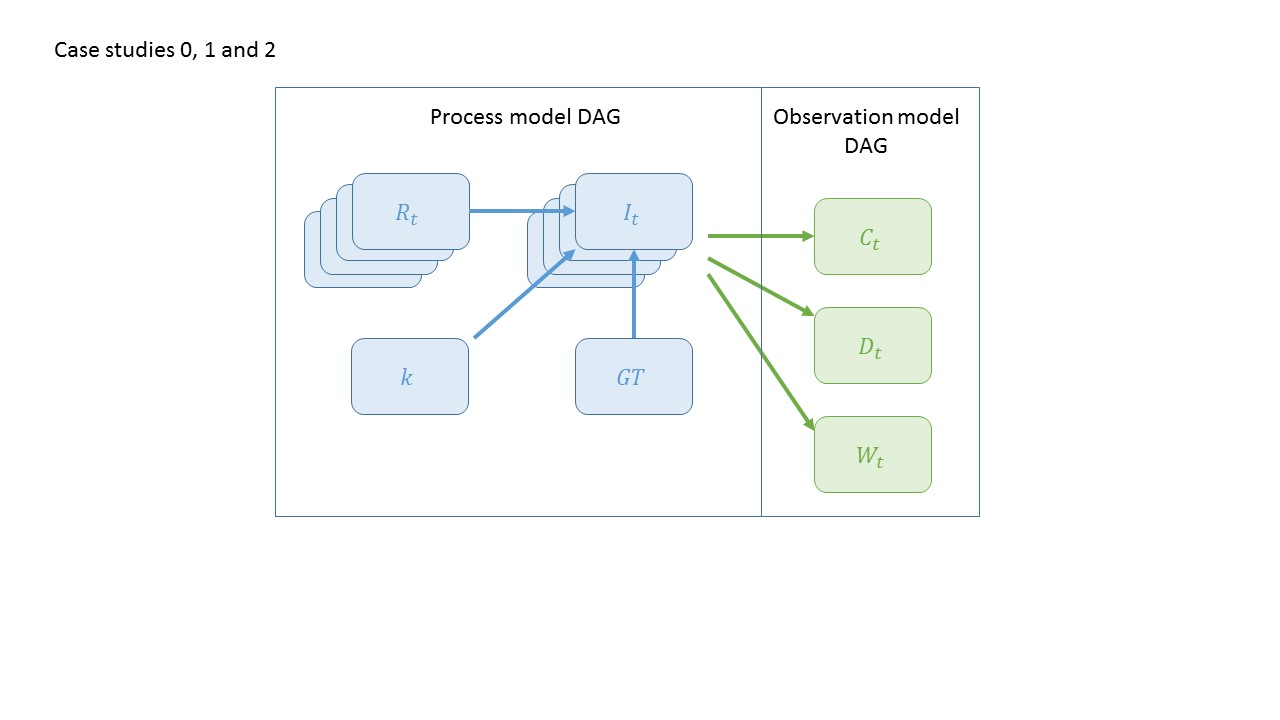
\includegraphics[width=0.75\textwidth]{figures/case_study_0_1_2.jpg}\\
(b)\\
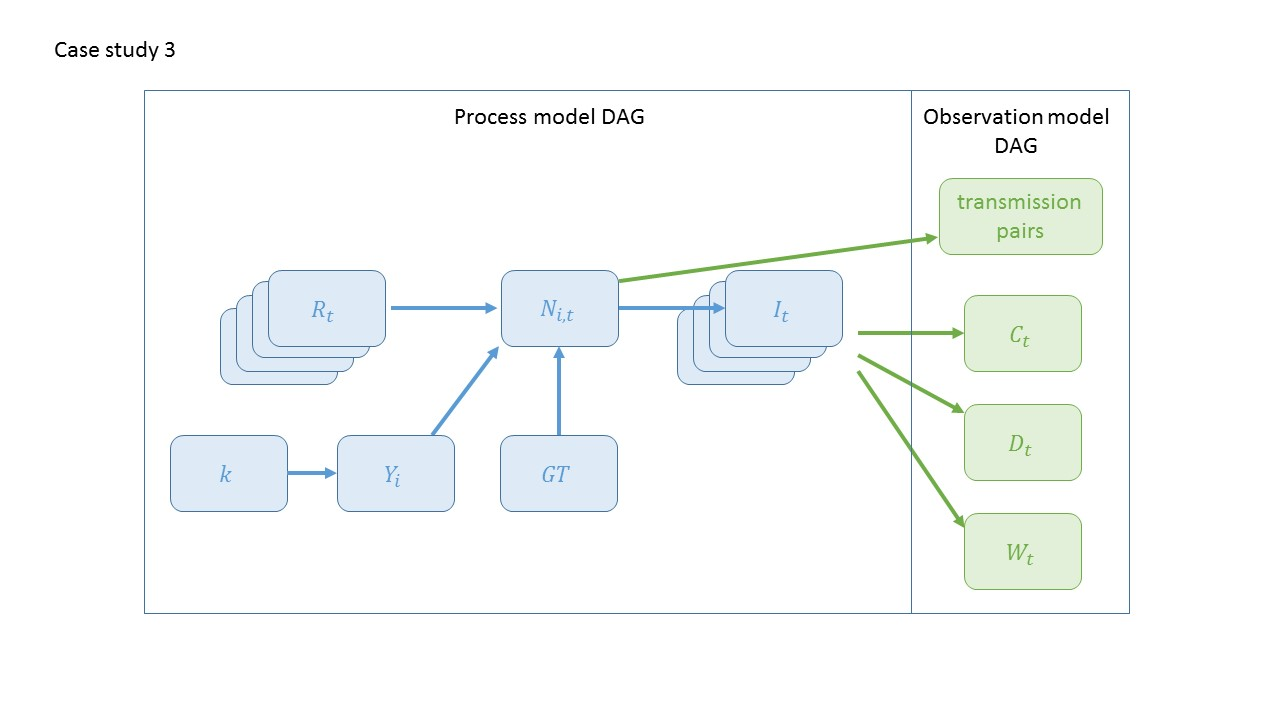
\includegraphics[width=0.75\textwidth]{figures/case_study_3.jpg}
\label{fig:CS3_DAG}
\caption{[Mike's attempt at DAGs for the case studies (can be made prettier later on).] Latent states in blue, observed states in green. (a) Case studies 0--2. Process model P1 is a special case where $I_t$ is a deterministic funcvtion of $R_t$ and $I_{1:t-1}$; P2 is a special case in the limit $k\to\infty$; P3 allowing the dispersion parameter $k$ to take any given value. The different observation models described in case study 0 (with or without underreporting, reporting delay, and observation noise) would affect how the expected value of the observed state $C_t$ relates to the latent states $I_{1:t}$, and the variance of the observed state $C_t$. Case studies 1 and 2 add additional observed states for deaths ($D_t$) and wasterwater observations ($W_t$) respectively. (b) Case study 3 requires more states to be inlcuded in the DAG to take account of individual heterogeneity and the impact it has on obsetved data on transmission pairs. The variable $N_{it}$ representing the number of secondary infections caused by individual $i$ on day $t$ encodes the full transmission tree. The expected value of $N_{it}$ is determined by the instantaneous reproduction number $R_t$, the relative transmission rates $Y_i$ of previously infected individuals, and their current infectiousness determined by the generation time distribution (GT). The variance in the distrubtion of $Y_i$ is determined by the dispersion parameter $k$.  }
\end{figure}






\section{Discussion}

\subsection{Summary}

We have presented a framework for integrating multiple data sources in infectious disease modelling that extends established Bayesian workflow principles.
This workflow serves both as guidance for practitioners developing multi-source models and as a checklist for readers evaluating modelling papers.
Our Bayesian workflow comprises linked steps that begin with data source characterisation using a structured checklist evaluating metadata, scope, resolution, data quality, data utility, and practical considerations.
Building from this foundation, we suggest defining research questions and target estimands that shape all downstream decisions.
We then recommend representing epidemiological mechanisms through process DAGs, with structure evolving as understanding improves during outbreaks.
Next, data source mapping connects surveillance streams to process components based on their expected contributions to target estimands.
Observation DAGs follow, linking latent processes to measured data through reporting mechanisms, delays, and biases.
Integration choices must then address what to combine and how, balancing theoretical benefits against practical constraints.
Fitting method selection completes the core workflow, balancing statistical rigor with computational feasibility across likelihood-based and likelihood-free approaches.
Throughout, feedback loops connect these stages because downstream constraints often require revisiting earlier assumptions.
During outbreaks and other evolving settings, analysts should regularly review their workflow choices as new data becomes available and adapt their methods when expecting rapid change or repeated analyses with similar model requirements.

Four case studies demonstrate this workflow using progressively more data sources for reproduction number estimation.
Each progression shows how additional data sources alter both process and observation DAGs whilst requiring new integration and fitting decisions.
We establish the baseline approach using case data to estimate $R_t$ whilst highlighting assumptions about generation time and reporting fractions.
Adding death data eliminates some reporting assumptions but shifts dependence to infection-to-death delay assumptions and requires new integration choices.
Wastewater data provides population-level signals independent of testing biases but requires understanding viral shedding processes and likelihood-free fitting methods.
Individual-level contact tracing enables direct overdispersion estimation but leads to hierarchical process models and latent variable approaches which can be computationally challenging.
Each case study also leads to new fitting choices and model validation strategies.
Throughout we highlight that considering each submodel in isolation is a useful starting point for model development and validation.
Each case study illustrates real-world trade-offs between model complexity, computational feasibility, and parameter identifiability.

\subsection{Strengths and Limitations/Outstanding Challenges}

A key strength of our suggested workflow is the explicit separation of epidemiological process DAGs from observation DAGs, recognising that these components draw from different domains: epidemiological processes are informed by infectious disease theory whilst observation models reflect data source characteristics and collection mechanisms.
This separation provides clarity for model development and validation.
The framework's applicability across diverse contexts, from early outbreak analysis to routine surveillance, offers flexibility for varied epidemiological questions.
In addition, our suggested data review process provides a structured approach to understanding different epidemiological data sources.
By providing explicit guidance on reporting standards, including validation procedures and code availability, we aim to improve both the development and evaluation of multi-source models.

Our suggested approach can be implemented with current tools, though doing so may require choosing between statistical rigour (resource-intensive joint models) and computational feasibility (pipeline approaches with known limitations).
The DAG-based workflow helps analysts plan for evolving data availability, but adapting models as surveillance systems change typically requires substantial rework.
Teams may need to maintain multiple parallel models for different data scenarios, potentially limiting rapid response capabilities.

Without shared infrastructure, teams typically rebuild common epidemiological processes for each application.
Current probabilistic programming frameworks provide foundations but often lack the epidemiological abstractions needed for routine use.
These implementation barriers can lead teams to adopt simpler approaches despite understanding their statistical limitations.

Workflow reporting remains inconsistent across the field, with varying levels of detail about model validation, code availability, and decision rationales.
Even when models are technically sound, incomplete reporting limits their utility for learning and adaptation.
Establishing community standards for workflow documentation would accelerate progress by enabling systematic learning from both successes and failures.

\subsection{Comparison with Existing Literature}
% TODO: Position relative to pipeline vs joint modelling literature
% TODO: Relationship to evidence synthesis and meta-analysis methods
% TODO: Comparison with ensemble forecasting approaches
% TODO: Distinguish from existing reviews and methodological papers
% TODO: Compare with other multi-source integration frameworks

Recent advances in machine learning-augmented fitting methods show promise, with neural network-based summary statistic construction \citep{raynal2019abc} and deep learning phylodynamic methods \citep{voznica2022deep}, providing alternatives to traditional likelihood evaluation. However, applying these methodological advances into the structured workflow framework we propose requires consideration of interpretability.

Recent work has made progress towards structured infectious disease modelling workflows, though implementation remains incomplete.
For example, \citet{bouman2024bayesian} systematically compared modelling choices for SARS-CoV-2 transmission and provided open-source implementation through their HETTMO package.
However, their approach, while methodologically sound, lacks the structured workflow guidance needed for broader application.
Key workflow elements such as prior predictive checks, systematic model criticism, and clear decision frameworks are absent.
Their work exemplifies the gap between implementing good models and following reproducible workflow practices.
In contrast, our framework provides explicit structured guidance through each workflow stage, with case studies demonstrating not just model implementation but the decision process itself.

\subsection{Future work}

Future progress requires infrastructure that bridges the gap between methodological best practice and routine implementation.
Whilst this paper provides a schematic workflow, a practical tutorial demonstrating actual implementation would provide essential guidance for practitioners.
Composable modelling tools, where individual self contained components can be combined to build more complex models, could enable modular development where domain experts contribute specialised components without rebuilding core functionality.
However, for such tutorials and tools to be tractable and useful, more work is needed on software composability and standardised interfaces.
Such tools would need standardised interfaces between model components, epidemiological abstractions for common processes, and support for seamless reconfiguration as data availability evolves.

Key priorities include developing community standards for model specification and validation across multiple data sources.
Computational scalability remains critical, particularly for joint analysis of individual-level genomic data with population surveillance.
As emerging data sources from digital health systems and environmental monitoring become available, frameworks must incorporate these streams whilst maintaining interpretability.
Model validation procedures that can detect conflicts between data sources and assess component compatibility need development beyond current approaches.
These advances would make rigorous multi-source integration accessible to public health teams without prohibitive resource requirements, enabling the rapid response capabilities that outbreak situations demand.


\section{Conclusions}

Infectious disease modelling workflows benefit from systematic approaches that can adapt to multiple data sources and evolving outbreak contexts.
We have presented workflow best practices that provide practical guidance for navigating trade-offs between information gain, computational complexity, and interpretability across diverse modelling scenarios.
Our workflow extends established Bayesian principles through structured steps from data characterisation to model validation, supported by expert consensus on data source characteristics and progressive case studies.
The modular approach we advocate enables practitioners to build complexity incrementally whilst maintaining transparency about modelling assumptions and integration choices.
We recommend that the infectious disease modelling community adopt these workflow best practices for both model development and evaluation.
Readers can use our framework as a systematic checklist when evaluating modelling papers to assess whether workflow choices are appropriate and transparent.
Practitioners should implement these approaches across all infectious disease modelling contexts, with particular value during rapidly evolving outbreaks where research questions shift and new data sources emerge.
Establishing community standards around systematic workflow practices will improve both methodological rigour and practical implementation across the field.

\section{Acknowledgements}

We thank the organisers and participants of the workshop "Analysis and modelling for the design of future epidemic surveillance systems" (CIRM, Marseille, 28 April–2 May 2025) for valuable discussions and feedback that helped shape this work.
We are particularly grateful to Anne Cori, Sebastian Funk, James McCaw, and Freya Shearer for organising this productive workshop.
All workshop participants provided useful discussion and feedback.
We thank Poppy the dog for making sure to ask the important questions.

\bibliographystyle{plainnat}
\bibliography{references,zotero-references}


\end{document}
 